\documentclass[1p]{elsarticle_modified}
%\bibliographystyle{elsarticle-num}

%\usepackage[colorlinks]{hyperref}
%\usepackage{abbrmath_seonhwa} %\Abb, \Ascr, \Acal ,\Abf, \Afrak
\usepackage{amsfonts}
\usepackage{amssymb}
\usepackage{amsmath}
\usepackage{amsthm}
\usepackage{scalefnt}
\usepackage{amsbsy}
\usepackage{kotex}
\usepackage{caption}
\usepackage{subfig}
\usepackage{color}
\usepackage{graphicx}
\usepackage{xcolor} %% white, black, red, green, blue, cyan, magenta, yellow
\usepackage{float}
\usepackage{setspace}
\usepackage{hyperref}

\usepackage{tikz}
\usetikzlibrary{arrows}

\usepackage{multirow}
\usepackage{array} % fixed length table
\usepackage{hhline}

%%%%%%%%%%%%%%%%%%%%%
\makeatletter
\renewcommand*\env@matrix[1][\arraystretch]{%
	\edef\arraystretch{#1}%
	\hskip -\arraycolsep
	\let\@ifnextchar\new@ifnextchar
	\array{*\c@MaxMatrixCols c}}
\makeatother %https://tex.stackexchange.com/questions/14071/how-can-i-increase-the-line-spacing-in-a-matrix
%%%%%%%%%%%%%%%

\usepackage[normalem]{ulem}

\newcommand{\msout}[1]{\ifmmode\text{\sout{\ensuremath{#1}}}\else\sout{#1}\fi}
%SOURCE: \msout is \stkout macro in https://tex.stackexchange.com/questions/20609/strikeout-in-math-mode

\newcommand{\cancel}[1]{
	\ifmmode
	{\color{red}\msout{#1}}
	\else
	{\color{red}\sout{#1}}
	\fi
}

\newcommand{\add}[1]{
	{\color{blue}\uwave{#1}}
}

\newcommand{\replace}[2]{
	\ifmmode
	{\color{red}\msout{#1}}{\color{blue}\uwave{#2}}
	\else
	{\color{red}\sout{#1}}{\color{blue}\uwave{#2}}
	\fi
}

\newcommand{\Sol}{\mathcal{S}} %segment
\newcommand{\D}{D} %diagram
\newcommand{\A}{\mathcal{A}} %arc


%%%%%%%%%%%%%%%%%%%%%%%%%%%%%5 test

\def\sl{\operatorname{\textup{SL}}(2,\Cbb)}
\def\psl{\operatorname{\textup{PSL}}(2,\Cbb)}
\def\quan{\mkern 1mu \triangleright \mkern 1mu}

\theoremstyle{definition}
\newtheorem{thm}{Theorem}[section]
\newtheorem{prop}[thm]{Proposition}
\newtheorem{lem}[thm]{Lemma}
\newtheorem{ques}[thm]{Question}
\newtheorem{cor}[thm]{Corollary}
\newtheorem{defn}[thm]{Definition}
\newtheorem{exam}[thm]{Example}
\newtheorem{rmk}[thm]{Remark}
\newtheorem{alg}[thm]{Algorithm}

\newcommand{\I}{\sqrt{-1}}
\begin{document}

%\begin{frontmatter}
%
%\title{Boundary parabolic representations of knots up to 8 crossings}
%
%%% Group authors per affiliation:
%\author{Yunhi Cho} 
%\address{Department of Mathematics, University of Seoul, Seoul, Korea}
%\ead{yhcho@uos.ac.kr}
%
%
%\author{Seonhwa Kim} %\fnref{s_kim}}
%\address{Center for Geometry and Physics, Institute for Basic Science, Pohang, 37673, Korea}
%\ead{ryeona17@ibs.re.kr}
%
%\author{Hyuk Kim}
%\address{Department of Mathematical Sciences, Seoul National University, Seoul 08826, Korea}
%\ead{hyukkim@snu.ac.kr}
%
%\author{Seokbeom Yoon}
%\address{Department of Mathematical Sciences, Seoul National University, Seoul, 08826,  Korea}
%\ead{sbyoon15@snu.ac.kr}
%
%\begin{abstract}
%We find all boundary parabolic representation of knots up to 8 crossings.
%
%\end{abstract}
%\begin{keyword}
%    \MSC[2010] 57M25 
%\end{keyword}
%
%\end{frontmatter}

%\linenumbers
%\tableofcontents
%
\newcommand\colored[1]{\textcolor{white}{\rule[-0.35ex]{0.8em}{1.4ex}}\kern-0.8em\color{red} #1}%
%\newcommand\colored[1]{\textcolor{white}{ #1}\kern-2.17ex	\textcolor{white}{ #1}\kern-1.81ex	\textcolor{white}{ #1}\kern-2.15ex\color{red}#1	}

{\Large $\underline{12a_{0483}~(K12a_{0483})}$}

\setlength{\tabcolsep}{10pt}
\renewcommand{\arraystretch}{1.6}
\vspace{1cm}\begin{tabular}{m{100pt}>{\centering\arraybackslash}m{274pt}}
\multirow{5}{120pt}{
	\centering
	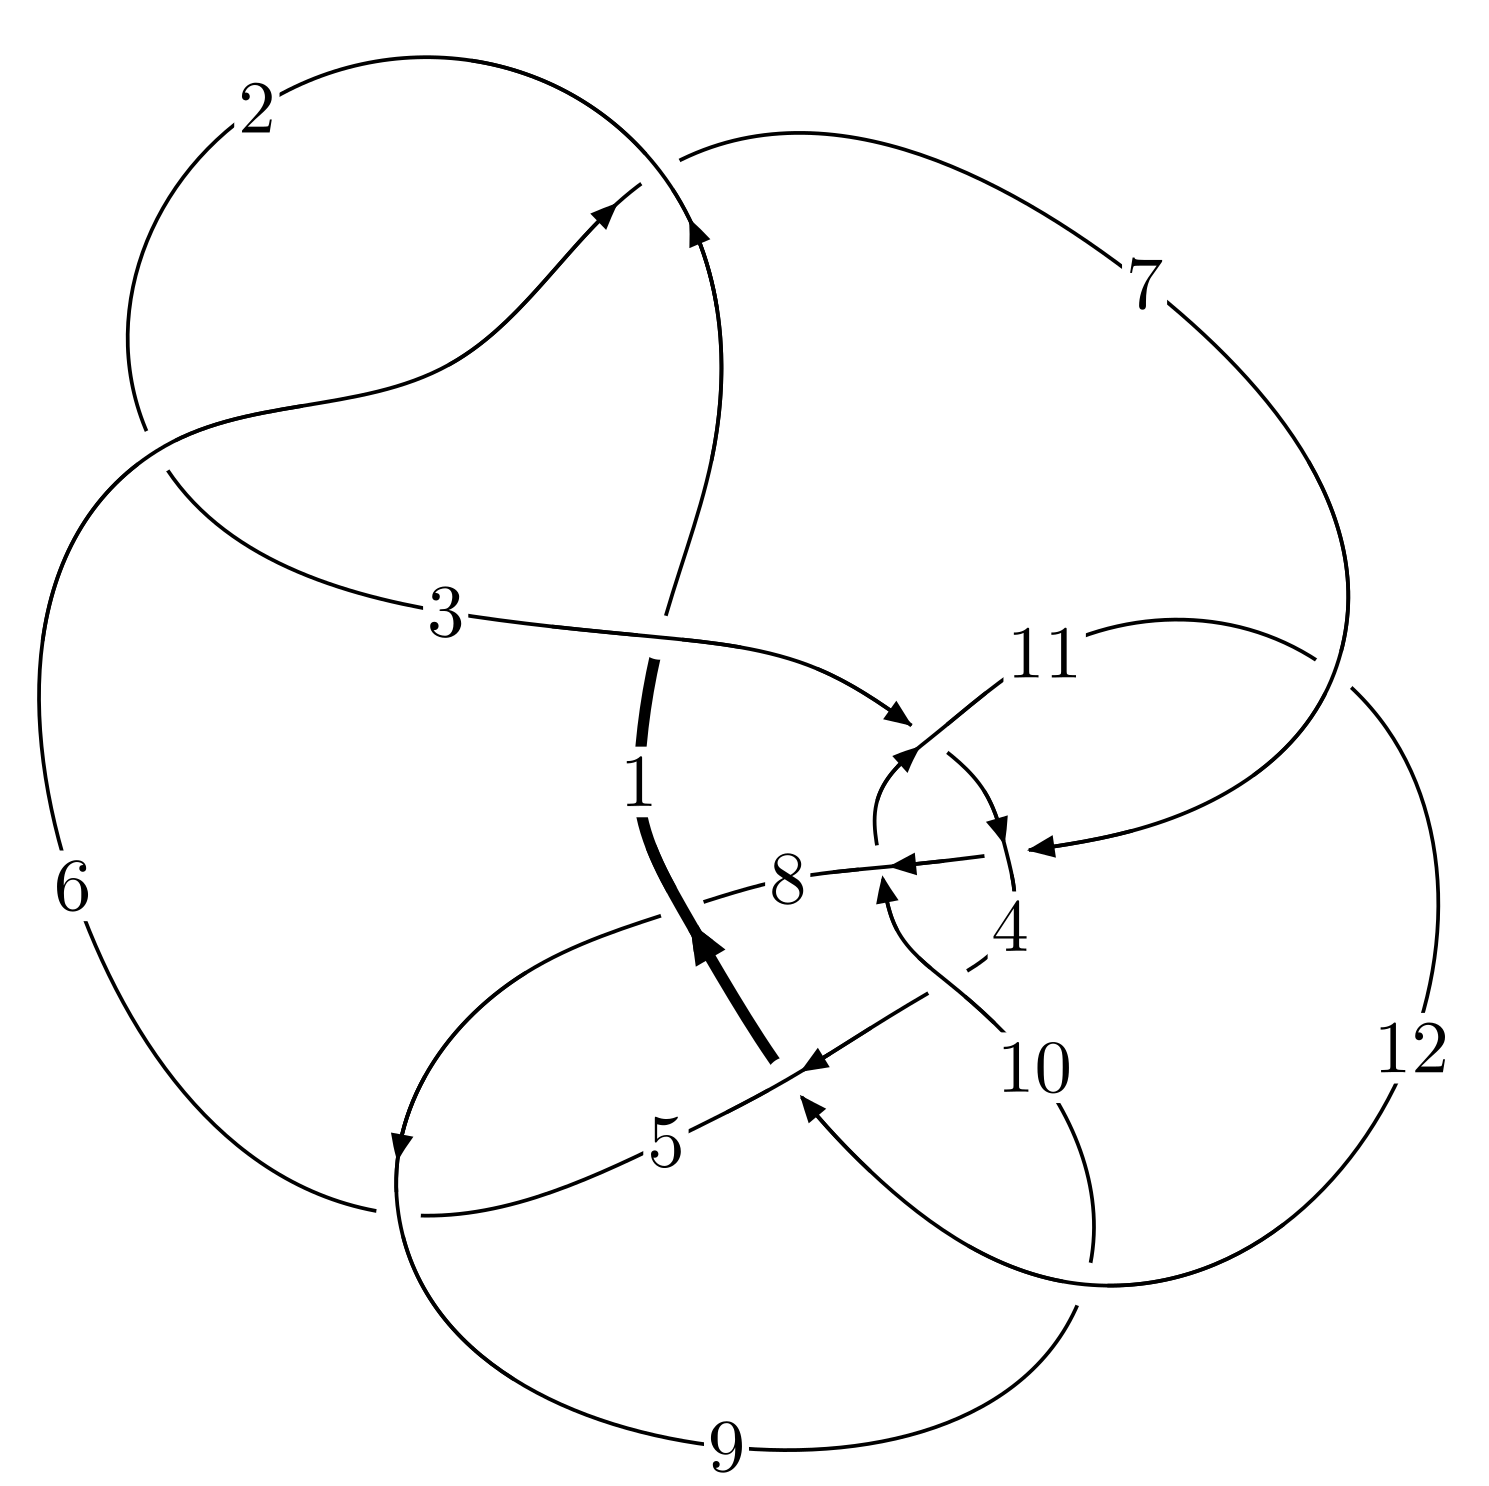
\includegraphics[width=112pt]{../../../GIT/diagram.site/Diagrams/png/1284_12a_0483.png}\\
\ \ \ A knot diagram\footnotemark}&
\allowdisplaybreaks
\textbf{Linearized knot diagam} \\
\cline{2-2}
 &
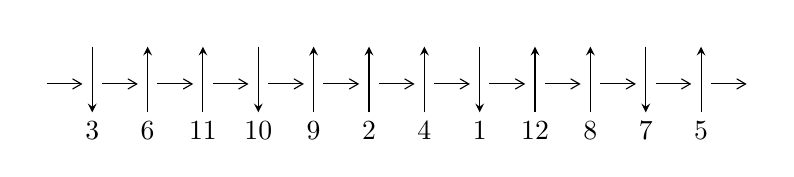
\begin{tikzpicture}[x=20pt, y=17pt]
	% nodes
	\node (C0) at (0, 0) {};
	\node (C1) at (1, 0) {};
	\node (C1U) at (1, +1) {};
	\node (C1D) at (1, -1) {3};

	\node (C2) at (2, 0) {};
	\node (C2U) at (2, +1) {};
	\node (C2D) at (2, -1) {6};

	\node (C3) at (3, 0) {};
	\node (C3U) at (3, +1) {};
	\node (C3D) at (3, -1) {11};

	\node (C4) at (4, 0) {};
	\node (C4U) at (4, +1) {};
	\node (C4D) at (4, -1) {10};

	\node (C5) at (5, 0) {};
	\node (C5U) at (5, +1) {};
	\node (C5D) at (5, -1) {9};

	\node (C6) at (6, 0) {};
	\node (C6U) at (6, +1) {};
	\node (C6D) at (6, -1) {2};

	\node (C7) at (7, 0) {};
	\node (C7U) at (7, +1) {};
	\node (C7D) at (7, -1) {4};

	\node (C8) at (8, 0) {};
	\node (C8U) at (8, +1) {};
	\node (C8D) at (8, -1) {1};

	\node (C9) at (9, 0) {};
	\node (C9U) at (9, +1) {};
	\node (C9D) at (9, -1) {12};

	\node (C10) at (10, 0) {};
	\node (C10U) at (10, +1) {};
	\node (C10D) at (10, -1) {8};

	\node (C11) at (11, 0) {};
	\node (C11U) at (11, +1) {};
	\node (C11D) at (11, -1) {7};

	\node (C12) at (12, 0) {};
	\node (C12U) at (12, +1) {};
	\node (C12D) at (12, -1) {5};
	\node (C13) at (13, 0) {};

	% arrows
	\draw[->,>={angle 60}]
	(C0) edge (C1) (C1) edge (C2) (C2) edge (C3) (C3) edge (C4) (C4) edge (C5) (C5) edge (C6) (C6) edge (C7) (C7) edge (C8) (C8) edge (C9) (C9) edge (C10) (C10) edge (C11) (C11) edge (C12) (C12) edge (C13) ;	\draw[->,>=stealth]
	(C1U) edge (C1D) (C2D) edge (C2U) (C3D) edge (C3U) (C4U) edge (C4D) (C5D) edge (C5U) (C6D) edge (C6U) (C7D) edge (C7U) (C8U) edge (C8D) (C9D) edge (C9U) (C10D) edge (C10U) (C11U) edge (C11D) (C12D) edge (C12U) ;
	\end{tikzpicture} \\
\hhline{~~} \\& 
\textbf{Solving Sequence} \\ \cline{2-2} 
 &
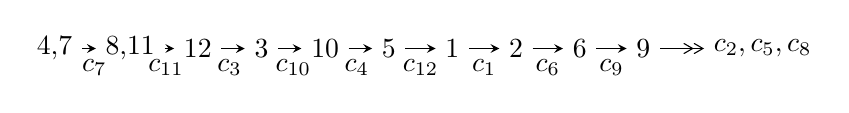
\begin{tikzpicture}[x=23pt, y=7pt]
	% node
	\node (A0) at (-1/8, 0) {4,7};
	\node (A1) at (17/16, 0) {8,11};
	\node (A2) at (17/8, 0) {12};
	\node (A3) at (25/8, 0) {3};
	\node (A4) at (33/8, 0) {10};
	\node (A5) at (41/8, 0) {5};
	\node (A6) at (49/8, 0) {1};
	\node (A7) at (57/8, 0) {2};
	\node (A8) at (65/8, 0) {6};
	\node (A9) at (73/8, 0) {9};
	\node (C1) at (1/2, -1) {$c_{7}$};
	\node (C2) at (13/8, -1) {$c_{11}$};
	\node (C3) at (21/8, -1) {$c_{3}$};
	\node (C4) at (29/8, -1) {$c_{10}$};
	\node (C5) at (37/8, -1) {$c_{4}$};
	\node (C6) at (45/8, -1) {$c_{12}$};
	\node (C7) at (53/8, -1) {$c_{1}$};
	\node (C8) at (61/8, -1) {$c_{6}$};
	\node (C9) at (69/8, -1) {$c_{9}$};
	\node (A10) at (11, 0) {$c_{2},c_{5},c_{8}$};

	% edge
	\draw[->,>=stealth]	
	(A0) edge (A1) (A1) edge (A2) (A2) edge (A3) (A3) edge (A4) (A4) edge (A5) (A5) edge (A6) (A6) edge (A7) (A7) edge (A8) (A8) edge (A9) ;
	\draw[->>,>={angle 60}]	
	(A9) edge (A10);
\end{tikzpicture} \\ 

\end{tabular} \\

\footnotetext{
The image of knot diagram is generated by the software ``\textbf{Draw programme}" developed by Andrew Bartholomew(\url{http://www.layer8.co.uk/maths/draw/index.htm\#Running-draw}), where we modified some parts for our purpose(\url{https://github.com/CATsTAILs/LinksPainter}).
}\phantom \\ \newline 
\centering \textbf{Ideals for irreducible components\footnotemark of $X_{\text{par}}$} 
 
\begin{align*}
I^u_{1}&=\langle 
3.39637\times10^{102} u^{49}+9.37271\times10^{101} u^{48}+\cdots+4.22304\times10^{102} b-4.54172\times10^{103},\\
\phantom{I^u_{1}}&\phantom{= \langle  }5.05934\times10^{103} u^{49}-2.24413\times10^{104} u^{48}+\cdots+2.06929\times10^{104} a-6.26286\times10^{105},\;u^{50}+u^{49}+\cdots-13 u+7\rangle \\
I^u_{2}&=\langle 
1.21305\times10^{1409} u^{169}-2.95236\times10^{1409} u^{168}+\cdots+2.55035\times10^{1408} b-2.02591\times10^{1409},\\
\phantom{I^u_{2}}&\phantom{= \langle  }-1.12706\times10^{1409} u^{169}+2.73180\times10^{1409} u^{168}+\cdots+2.55035\times10^{1408} a+3.50626\times10^{1409},\\
\phantom{I^u_{2}}&\phantom{= \langle  }u^{170}-3 u^{169}+\cdots-4 u+1\rangle \\
I^u_{3}&=\langle 
1.74194\times10^{110} u^{45}-1.94041\times10^{110} u^{44}+\cdots+1.58393\times10^{111} b-1.73190\times10^{111},\\
\phantom{I^u_{3}}&\phantom{= \langle  }-5.80551\times10^{111} u^{45}+4.76976\times10^{111} u^{44}+\cdots+1.10875\times10^{112} a+7.13483\times10^{112},\;u^{46}- u^{45}+\cdots-7 u+7\rangle \\
I^u_{4}&=\langle 
- u^8+2 u^6+2 u^5- u^4- u^3-4 u^2+b+3,\;- u^8+2 u^6+2 u^5- u^4- u^3-4 u^2+a+4,\\
\phantom{I^u_{4}}&\phantom{= \langle  }u^9+u^8- u^7-3 u^6-2 u^5- u^4+3 u^3+3 u^2- u-1\rangle \\
I^u_{5}&=\langle 
b-1,\;a-1,\;u^2+u+1\rangle \\
\\
\end{align*}
\raggedright * 5 irreducible components of $\dim_{\mathbb{C}}=0$, with total 277 representations.\\
\footnotetext{All coefficients of polynomials are rational numbers. But the coefficients are sometimes approximated in decimal forms when there is not enough margin.}
\newpage
\renewcommand{\arraystretch}{1}
\centering \section*{I. $I^u_{1}= \langle 3.40\times10^{102} u^{49}+9.37\times10^{101} u^{48}+\cdots+4.22\times10^{102} b-4.54\times10^{103},\;5.06\times10^{103} u^{49}-2.24\times10^{104} u^{48}+\cdots+2.07\times10^{104} a-6.26\times10^{105},\;u^{50}+u^{49}+\cdots-13 u+7 \rangle$}
\flushleft \textbf{(i) Arc colorings}\\
\begin{tabular}{m{7pt} m{180pt} m{7pt} m{180pt} }
\flushright $a_{4}=$&$\begin{pmatrix}0\\u\end{pmatrix}$ \\
\flushright $a_{7}=$&$\begin{pmatrix}1\\0\end{pmatrix}$ \\
\flushright $a_{8}=$&$\begin{pmatrix}1\\- u^2\end{pmatrix}$ \\
\flushright $a_{11}=$&$\begin{pmatrix}-0.244496 u^{49}+1.08449 u^{48}+\cdots-64.7799 u+30.2657\\-0.804246 u^{49}-0.221942 u^{48}+\cdots-39.0383 u+10.7546\end{pmatrix}$ \\
\flushright $a_{12}=$&$\begin{pmatrix}0.559750 u^{49}+1.30643 u^{48}+\cdots-25.7416 u+19.5111\\-0.804246 u^{49}-0.221942 u^{48}+\cdots-39.0383 u+10.7546\end{pmatrix}$ \\
\flushright $a_{3}=$&$\begin{pmatrix}-3.61778 u^{49}-5.22963 u^{48}+\cdots-7.96421 u-42.2363\\-0.982837 u^{49}-1.60843 u^{48}+\cdots+10.0119 u-14.6152\end{pmatrix}$ \\
\flushright $a_{10}=$&$\begin{pmatrix}0.482332 u^{49}+1.62160 u^{48}+\cdots-44.7299 u+28.8140\\-0.567388 u^{49}-0.0819737 u^{48}+\cdots-31.4842 u+9.42658\end{pmatrix}$ \\
\flushright $a_{5}=$&$\begin{pmatrix}-4.54858 u^{49}-5.81641 u^{48}+\cdots-47.1344 u-34.9858\\-0.558867 u^{49}-1.04551 u^{48}+\cdots+11.4296 u-12.7931\end{pmatrix}$ \\
\flushright $a_{1}=$&$\begin{pmatrix}1.82758 u^{49}+1.26871 u^{48}+\cdots+68.3757 u-12.3290\\-0.317601 u^{49}+0.0639091 u^{48}+\cdots-18.9800 u+6.84255\end{pmatrix}$ \\
\flushright $a_{2}=$&$\begin{pmatrix}0.627463 u^{49}+3.27508 u^{48}+\cdots-105.094 u+60.7596\\-0.269618 u^{49}+0.509041 u^{48}+\cdots-44.5208 u+16.3153\end{pmatrix}$ \\
\flushright $a_{6}=$&$\begin{pmatrix}-2.01281 u^{49}-2.50341 u^{48}+\cdots-25.2865 u-15.7923\\1.38953 u^{49}+1.23474 u^{48}+\cdots+34.4210 u-4.49427\end{pmatrix}$ \\
\flushright $a_{9}=$&$\begin{pmatrix}0.0910837 u^{49}+0.454900 u^{48}+\cdots-18.0495 u+11.5917\\-0.652183 u^{49}+0.424567 u^{48}+\cdots-50.4902 u+19.4551\end{pmatrix}$\\&\end{tabular}
\flushleft \textbf{(ii) Obstruction class $= -1$}\\~\\
\flushleft \textbf{(iii) Cusp Shapes $= -1.91113 u^{49}-0.862109 u^{48}+\cdots-86.2208 u+16.6705$}\\~\\
\newpage\renewcommand{\arraystretch}{1}
\flushleft \textbf{(iv) u-Polynomials at the component}\newline \\
\begin{tabular}{m{50pt}|m{274pt}}
Crossings & \hspace{64pt}u-Polynomials at each crossing \\
\hline $$\begin{aligned}c_{1}\end{aligned}$$&$\begin{aligned}
&u^{50}+26 u^{49}+\cdots+10532 u+1296
\end{aligned}$\\
\hline $$\begin{aligned}c_{2},c_{6}\end{aligned}$$&$\begin{aligned}
&u^{50}-4 u^{49}+\cdots-94 u+36
\end{aligned}$\\
\hline $$\begin{aligned}c_{3},c_{5}\end{aligned}$$&$\begin{aligned}
&7(7 u^{50}- u^{49}+\cdots- u+1)
\end{aligned}$\\
\hline $$\begin{aligned}c_{4}\end{aligned}$$&$\begin{aligned}
&7(7 u^{50}-29 u^{49}+\cdots-10240 u+2048)
\end{aligned}$\\
\hline $$\begin{aligned}c_{7},c_{12}\end{aligned}$$&$\begin{aligned}
&u^{50}+u^{49}+\cdots-13 u+7
\end{aligned}$\\
\hline $$\begin{aligned}c_{8},c_{11}\end{aligned}$$&$\begin{aligned}
&u^{50}-12 u^{49}+\cdots-800 u+56
\end{aligned}$\\
\hline $$\begin{aligned}c_{9},c_{10}\end{aligned}$$&$\begin{aligned}
&u^{50}-7 u^{49}+\cdots+3 u+1
\end{aligned}$\\
\hline
\end{tabular}\\~\\
\newpage\renewcommand{\arraystretch}{1}
\flushleft \textbf{(v) Riley Polynomials at the component}\newline \\
\begin{tabular}{m{50pt}|m{274pt}}
Crossings & \hspace{64pt}Riley Polynomials at each crossing \\
\hline $$\begin{aligned}c_{1}\end{aligned}$$&$\begin{aligned}
&y^{50}-2 y^{49}+\cdots+8736656 y+1679616
\end{aligned}$\\
\hline $$\begin{aligned}c_{2},c_{6}\end{aligned}$$&$\begin{aligned}
&y^{50}+26 y^{49}+\cdots+10532 y+1296
\end{aligned}$\\
\hline $$\begin{aligned}c_{3},c_{5}\end{aligned}$$&$\begin{aligned}
&49(49 y^{50}-771 y^{49}+\cdots+7 y+1)
\end{aligned}$\\
\hline $$\begin{aligned}c_{4}\end{aligned}$$&$\begin{aligned}
&49(49 y^{50}-379 y^{49}+\cdots+1.30023\times10^{8} y+4194304)
\end{aligned}$\\
\hline $$\begin{aligned}c_{7},c_{12}\end{aligned}$$&$\begin{aligned}
&y^{50}+11 y^{49}+\cdots+545 y+49
\end{aligned}$\\
\hline $$\begin{aligned}c_{8},c_{11}\end{aligned}$$&$\begin{aligned}
&y^{50}+2 y^{49}+\cdots+69184 y+3136
\end{aligned}$\\
\hline $$\begin{aligned}c_{9},c_{10}\end{aligned}$$&$\begin{aligned}
&y^{50}+3 y^{49}+\cdots-13 y+1
\end{aligned}$\\
\hline
\end{tabular}\\~\\
\newpage\flushleft \textbf{(vi) Complex Volumes and Cusp Shapes}
$$\begin{array}{c|c|c}  
\text{Solutions to }I^u_{1}& \I (\text{vol} + \sqrt{-1}CS) & \text{Cusp shape}\\
 \hline 
\begin{aligned}
u &= \phantom{-}0.896598 + 0.225500 I \\
a &= -0.780358 - 0.128987 I \\
b &= -0.183649 - 0.899545 I\end{aligned}
 & \phantom{-}1.31909 + 6.48073 I & \phantom{-}9.60802 - 9.06692 I \\ \hline\begin{aligned}
u &= \phantom{-}0.896598 - 0.225500 I \\
a &= -0.780358 + 0.128987 I \\
b &= -0.183649 + 0.899545 I\end{aligned}
 & \phantom{-}1.31909 - 6.48073 I & \phantom{-}9.60802 + 9.06692 I \\ \hline\begin{aligned}
u &= \phantom{-}0.587053 + 0.920652 I \\
a &= -1.48929 + 0.43644 I \\
b &= -0.699778 + 0.870114 I\end{aligned}
 & -0.79150 + 7.68128 I & \phantom{-}1.82344 - 9.07192 I \\ \hline\begin{aligned}
u &= \phantom{-}0.587053 - 0.920652 I \\
a &= -1.48929 - 0.43644 I \\
b &= -0.699778 - 0.870114 I\end{aligned}
 & -0.79150 - 7.68128 I & \phantom{-}1.82344 + 9.07192 I \\ \hline\begin{aligned}
u &= -0.650166 + 0.908574 I \\
a &= -1.62557 - 0.20441 I \\
b &= -0.824128 - 0.959289 I\end{aligned}
 & -3.16337 - 13.32280 I & \phantom{-0.000000 -}0. + 12.11892 I \\ \hline\begin{aligned}
u &= -0.650166 - 0.908574 I \\
a &= -1.62557 + 0.20441 I \\
b &= -0.824128 + 0.959289 I\end{aligned}
 & -3.16337 + 13.32280 I & \phantom{-0.000000 } 0. - 12.11892 I \\ \hline\begin{aligned}
u &= \phantom{-}0.390507 + 1.111150 I \\
a &= -0.138073 - 0.218677 I \\
b &= -0.924397 - 0.924224 I\end{aligned}
 & -0.151526 + 1.007590 I & \phantom{-0.000000 } 0 \\ \hline\begin{aligned}
u &= \phantom{-}0.390507 - 1.111150 I \\
a &= -0.138073 + 0.218677 I \\
b &= -0.924397 + 0.924224 I\end{aligned}
 & -0.151526 - 1.007590 I & \phantom{-0.000000 } 0 \\ \hline\begin{aligned}
u &= \phantom{-}0.201424 + 0.796208 I \\
a &= -0.48677 + 1.73037 I \\
b &= -0.217057 + 0.628022 I\end{aligned}
 & \phantom{-}1.68069 + 3.72688 I & \phantom{-}0.72867 - 11.46445 I \\ \hline\begin{aligned}
u &= \phantom{-}0.201424 - 0.796208 I \\
a &= -0.48677 - 1.73037 I \\
b &= -0.217057 - 0.628022 I\end{aligned}
 & \phantom{-}1.68069 - 3.72688 I & \phantom{-}0.72867 + 11.46445 I\\
 \hline 
 \end{array}$$\newpage$$\begin{array}{c|c|c}  
\text{Solutions to }I^u_{1}& \I (\text{vol} + \sqrt{-1}CS) & \text{Cusp shape}\\
 \hline 
\begin{aligned}
u &= -0.217536 + 1.210190 I \\
a &= -0.294866 + 0.348219 I \\
b &= -1.43371 + 1.09461 I\end{aligned}
 & -1.98809 + 4.07284 I & \phantom{-0.000000 } 0 \\ \hline\begin{aligned}
u &= -0.217536 - 1.210190 I \\
a &= -0.294866 - 0.348219 I \\
b &= -1.43371 - 1.09461 I\end{aligned}
 & -1.98809 - 4.07284 I & \phantom{-0.000000 } 0 \\ \hline\begin{aligned}
u &= -0.578213 + 1.092660 I \\
a &= -0.950662 - 0.265934 I \\
b &= -0.754719 - 0.548695 I\end{aligned}
 & -6.65501 - 4.42416 I & \phantom{-0.000000 } 0 \\ \hline\begin{aligned}
u &= -0.578213 - 1.092660 I \\
a &= -0.950662 + 0.265934 I \\
b &= -0.754719 + 0.548695 I\end{aligned}
 & -6.65501 + 4.42416 I & \phantom{-0.000000 } 0 \\ \hline\begin{aligned}
u &= -0.703946 + 0.215017 I \\
a &= -1.157320 - 0.212380 I \\
b &= -0.387036 + 0.904155 I\end{aligned}
 & \phantom{-}3.43084 - 2.52625 I & \phantom{-}14.5793 + 4.3406 I \\ \hline\begin{aligned}
u &= -0.703946 - 0.215017 I \\
a &= -1.157320 + 0.212380 I \\
b &= -0.387036 - 0.904155 I\end{aligned}
 & \phantom{-}3.43084 + 2.52625 I & \phantom{-}14.5793 - 4.3406 I \\ \hline\begin{aligned}
u &= -0.039429 + 0.676536 I \\
a &= \phantom{-}1.108780 + 0.614567 I \\
b &= \phantom{-}0.74487 + 1.35597 I\end{aligned}
 & -2.15722 - 7.10901 I & -1.75060 + 10.31895 I \\ \hline\begin{aligned}
u &= -0.039429 - 0.676536 I \\
a &= \phantom{-}1.108780 - 0.614567 I \\
b &= \phantom{-}0.74487 - 1.35597 I\end{aligned}
 & -2.15722 + 7.10901 I & -1.75060 - 10.31895 I \\ \hline\begin{aligned}
u &= \phantom{-}0.104668 + 0.657602 I \\
a &= \phantom{-}1.015970 - 0.352637 I \\
b &= \phantom{-}0.440762 - 1.095320 I\end{aligned}
 & \phantom{-}0.03228 + 2.37617 I & \phantom{-}2.05698 - 5.41529 I \\ \hline\begin{aligned}
u &= \phantom{-}0.104668 - 0.657602 I \\
a &= \phantom{-}1.015970 + 0.352637 I \\
b &= \phantom{-}0.440762 + 1.095320 I\end{aligned}
 & \phantom{-}0.03228 - 2.37617 I & \phantom{-}2.05698 + 5.41529 I\\
 \hline 
 \end{array}$$\newpage$$\begin{array}{c|c|c}  
\text{Solutions to }I^u_{1}& \I (\text{vol} + \sqrt{-1}CS) & \text{Cusp shape}\\
 \hline 
\begin{aligned}
u &= \phantom{-}0.425932 + 0.502432 I \\
a &= \phantom{-}0.218708 + 0.840394 I \\
b &= -0.260537 - 0.727531 I\end{aligned}
 & \phantom{-}0.65061 + 1.83401 I & \phantom{-}2.77271 - 2.66351 I \\ \hline\begin{aligned}
u &= \phantom{-}0.425932 - 0.502432 I \\
a &= \phantom{-}0.218708 - 0.840394 I \\
b &= -0.260537 + 0.727531 I\end{aligned}
 & \phantom{-}0.65061 - 1.83401 I & \phantom{-}2.77271 + 2.66351 I \\ \hline\begin{aligned}
u &= -0.032968 + 1.352720 I \\
a &= -0.600335 + 0.087933 I \\
b &= -2.30156 + 0.26457 I\end{aligned}
 & -4.21497 - 1.45791 I & \phantom{-0.000000 } 0 \\ \hline\begin{aligned}
u &= -0.032968 - 1.352720 I \\
a &= -0.600335 - 0.087933 I \\
b &= -2.30156 - 0.26457 I\end{aligned}
 & -4.21497 + 1.45791 I & \phantom{-0.000000 } 0 \\ \hline\begin{aligned}
u &= -0.033602 + 0.587650 I \\
a &= \phantom{-}1.41694 + 0.29361 I \\
b &= \phantom{-}0.970954 + 0.649194 I\end{aligned}
 & -3.92153 + 0.23254 I & -2.51689 + 2.55719 I \\ \hline\begin{aligned}
u &= -0.033602 - 0.587650 I \\
a &= \phantom{-}1.41694 - 0.29361 I \\
b &= \phantom{-}0.970954 - 0.649194 I\end{aligned}
 & -3.92153 - 0.23254 I & -2.51689 - 2.55719 I \\ \hline\begin{aligned}
u &= \phantom{-}1.15136 + 0.83842 I \\
a &= \phantom{-}0.378166 - 0.327378 I \\
b &= -0.565487 - 0.444689 I\end{aligned}
 & \phantom{-}1.99652 + 0.43267 I & \phantom{-0.000000 } 0 \\ \hline\begin{aligned}
u &= \phantom{-}1.15136 - 0.83842 I \\
a &= \phantom{-}0.378166 + 0.327378 I \\
b &= -0.565487 + 0.444689 I\end{aligned}
 & \phantom{-}1.99652 - 0.43267 I & \phantom{-0.000000 } 0 \\ \hline\begin{aligned}
u &= -0.548514 + 0.133009 I \\
a &= -2.08340 - 0.61728 I \\
b &= -0.673485 + 0.793936 I\end{aligned}
 & \phantom{-}3.75232 - 1.50137 I & \phantom{-}11.49576 + 2.69889 I \\ \hline\begin{aligned}
u &= -0.548514 - 0.133009 I \\
a &= -2.08340 + 0.61728 I \\
b &= -0.673485 - 0.793936 I\end{aligned}
 & \phantom{-}3.75232 + 1.50137 I & \phantom{-}11.49576 - 2.69889 I\\
 \hline 
 \end{array}$$\newpage$$\begin{array}{c|c|c}  
\text{Solutions to }I^u_{1}& \I (\text{vol} + \sqrt{-1}CS) & \text{Cusp shape}\\
 \hline 
\begin{aligned}
u &= -0.013356 + 0.533801 I \\
a &= \phantom{-}1.72298 - 2.56125 I \\
b &= -0.050304 - 0.503806 I\end{aligned}
 & \phantom{-}1.49160 + 1.65153 I & -4.74713 - 1.23852 I \\ \hline\begin{aligned}
u &= -0.013356 - 0.533801 I \\
a &= \phantom{-}1.72298 + 2.56125 I \\
b &= -0.050304 + 0.503806 I\end{aligned}
 & \phantom{-}1.49160 - 1.65153 I & -4.74713 + 1.23852 I \\ \hline\begin{aligned}
u &= -0.81574 + 1.23486 I \\
a &= -0.257474 + 0.032226 I \\
b &= -0.607824 + 0.343957 I\end{aligned}
 & -5.73972 - 3.90228 I & \phantom{-0.000000 } 0 \\ \hline\begin{aligned}
u &= -0.81574 - 1.23486 I \\
a &= -0.257474 - 0.032226 I \\
b &= -0.607824 - 0.343957 I\end{aligned}
 & -5.73972 + 3.90228 I & \phantom{-0.000000 } 0 \\ \hline\begin{aligned}
u &= \phantom{-}0.484055 + 0.071183 I \\
a &= -3.03028 + 0.60100 I \\
b &= -0.924312 - 0.588508 I\end{aligned}
 & \phantom{-}2.19104 - 2.78946 I & \phantom{-}2.06202 + 2.65818 I \\ \hline\begin{aligned}
u &= \phantom{-}0.484055 - 0.071183 I \\
a &= -3.03028 - 0.60100 I \\
b &= -0.924312 + 0.588508 I\end{aligned}
 & \phantom{-}2.19104 + 2.78946 I & \phantom{-}2.06202 - 2.65818 I \\ \hline\begin{aligned}
u &= \phantom{-}1.18638 + 1.01584 I \\
a &= \phantom{-}1.047690 + 0.160806 I \\
b &= \phantom{-}1.20084 - 1.34273 I\end{aligned}
 & \phantom{-}0.3645 + 22.4198 I & \phantom{-0.000000 } 0 \\ \hline\begin{aligned}
u &= \phantom{-}1.18638 - 1.01584 I \\
a &= \phantom{-}1.047690 - 0.160806 I \\
b &= \phantom{-}1.20084 + 1.34273 I\end{aligned}
 & \phantom{-}0.3645 - 22.4198 I & \phantom{-0.000000 } 0 \\ \hline\begin{aligned}
u &= -1.19437 + 1.02640 I \\
a &= \phantom{-}0.999670 - 0.103934 I \\
b &= \phantom{-}1.04609 + 1.32397 I\end{aligned}
 & \phantom{-}2.9161 - 16.6430 I & \phantom{-0.000000 } 0 \\ \hline\begin{aligned}
u &= -1.19437 - 1.02640 I \\
a &= \phantom{-}0.999670 + 0.103934 I \\
b &= \phantom{-}1.04609 - 1.32397 I\end{aligned}
 & \phantom{-}2.9161 + 16.6430 I & \phantom{-0.000000 } 0\\
 \hline 
 \end{array}$$\newpage$$\begin{array}{c|c|c}  
\text{Solutions to }I^u_{1}& \I (\text{vol} + \sqrt{-1}CS) & \text{Cusp shape}\\
 \hline 
\begin{aligned}
u &= \phantom{-}1.22683 + 1.02462 I \\
a &= \phantom{-}0.857192 + 0.139921 I \\
b &= \phantom{-}0.950039 - 1.040830 I\end{aligned}
 & -2.99524 + 13.00340 I & \phantom{-0.000000 } 0 \\ \hline\begin{aligned}
u &= \phantom{-}1.22683 - 1.02462 I \\
a &= \phantom{-}0.857192 - 0.139921 I \\
b &= \phantom{-}0.950039 + 1.040830 I\end{aligned}
 & -2.99524 - 13.00340 I & \phantom{-0.000000 } 0 \\ \hline\begin{aligned}
u &= -0.95568 + 1.28588 I \\
a &= \phantom{-}0.372125 + 0.282409 I \\
b &= -0.096825 + 0.533539 I\end{aligned}
 & -4.39828 - 4.21209 I & \phantom{-0.000000 } 0 \\ \hline\begin{aligned}
u &= -0.95568 - 1.28588 I \\
a &= \phantom{-}0.372125 - 0.282409 I \\
b &= -0.096825 - 0.533539 I\end{aligned}
 & -4.39828 + 4.21209 I & \phantom{-0.000000 } 0 \\ \hline\begin{aligned}
u &= -1.19497 + 1.08383 I \\
a &= \phantom{-}0.808624 + 0.146162 I \\
b &= \phantom{-}0.407539 + 1.244690 I\end{aligned}
 & \phantom{-}5.84680 - 11.93900 I & \phantom{-0.000000 } 0 \\ \hline\begin{aligned}
u &= -1.19497 - 1.08383 I \\
a &= \phantom{-}0.808624 - 0.146162 I \\
b &= \phantom{-}0.407539 - 1.244690 I\end{aligned}
 & \phantom{-}5.84680 + 11.93900 I & \phantom{-0.000000 } 0 \\ \hline\begin{aligned}
u &= \phantom{-}1.17365 + 1.11011 I \\
a &= \phantom{-}0.692252 - 0.242791 I \\
b &= \phantom{-}0.127090 - 1.119270 I\end{aligned}
 & \phantom{-}5.62915 + 5.55517 I & \phantom{-0.000000 } 0 \\ \hline\begin{aligned}
u &= \phantom{-}1.17365 - 1.11011 I \\
a &= \phantom{-}0.692252 + 0.242791 I \\
b &= \phantom{-}0.127090 + 1.119270 I\end{aligned}
 & \phantom{-}5.62915 - 5.55517 I & \phantom{-0.000000 } 0 \\ \hline\begin{aligned}
u &= -1.34998 + 1.18237 I \\
a &= \phantom{-}0.102241 + 0.382380 I \\
b &= -0.983384 + 0.387249 I\end{aligned}
 & -0.88229 + 5.54652 I & \phantom{-0.000000 } 0 \\ \hline\begin{aligned}
u &= -1.34998 - 1.18237 I \\
a &= \phantom{-}0.102241 - 0.382380 I \\
b &= -0.983384 - 0.387249 I\end{aligned}
 & -0.88229 - 5.54652 I & \phantom{-0.000000 } 0\\
 \hline 
 \end{array}$$\newpage\newpage\renewcommand{\arraystretch}{1}
\centering \section*{II. $I^u_{2}= \langle 1.21\times10^{1409} u^{169}-2.95\times10^{1409} u^{168}+\cdots+2.55\times10^{1408} b-2.03\times10^{1409},\;-1.13\times10^{1409} u^{169}+2.73\times10^{1409} u^{168}+\cdots+2.55\times10^{1408} a+3.51\times10^{1409},\;u^{170}-3 u^{169}+\cdots-4 u+1 \rangle$}
\flushleft \textbf{(i) Arc colorings}\\
\begin{tabular}{m{7pt} m{180pt} m{7pt} m{180pt} }
\flushright $a_{4}=$&$\begin{pmatrix}0\\u\end{pmatrix}$ \\
\flushright $a_{7}=$&$\begin{pmatrix}1\\0\end{pmatrix}$ \\
\flushright $a_{8}=$&$\begin{pmatrix}1\\- u^2\end{pmatrix}$ \\
\flushright $a_{11}=$&$\begin{pmatrix}4.41922 u^{169}-10.7115 u^{168}+\cdots+33.8521 u-13.7481\\-4.75640 u^{169}+11.5763 u^{168}+\cdots-12.6675 u+7.94363\end{pmatrix}$ \\
\flushright $a_{12}=$&$\begin{pmatrix}9.17561 u^{169}-22.2878 u^{168}+\cdots+46.5195 u-21.6918\\-4.75640 u^{169}+11.5763 u^{168}+\cdots-12.6675 u+7.94363\end{pmatrix}$ \\
\flushright $a_{3}=$&$\begin{pmatrix}-6.62580 u^{169}+18.1648 u^{168}+\cdots-86.8606 u+24.0352\\2.37647 u^{169}-5.90898 u^{168}+\cdots+10.5334 u-4.55519\end{pmatrix}$ \\
\flushright $a_{10}=$&$\begin{pmatrix}7.85716 u^{169}-18.9524 u^{168}+\cdots+40.7541 u-19.1456\\-5.98437 u^{169}+14.5434 u^{168}+\cdots-17.5214 u+10.0166\end{pmatrix}$ \\
\flushright $a_{5}=$&$\begin{pmatrix}-7.85674 u^{169}+21.1384 u^{168}+\cdots-91.0839 u+25.3133\\-0.647227 u^{169}+0.933675 u^{168}+\cdots-2.21501 u-0.867296\end{pmatrix}$ \\
\flushright $a_{1}=$&$\begin{pmatrix}-12.1111 u^{169}+30.3758 u^{168}+\cdots+8.99007 u+19.7552\\3.83118 u^{169}-9.20539 u^{168}+\cdots+20.5805 u-5.14637\end{pmatrix}$ \\
\flushright $a_{2}=$&$\begin{pmatrix}10.1660 u^{169}-25.3071 u^{168}+\cdots+90.3787 u-19.6312\\-0.789997 u^{169}+1.86097 u^{168}+\cdots-1.96231 u+1.29485\end{pmatrix}$ \\
\flushright $a_{6}=$&$\begin{pmatrix}-6.73253 u^{169}+17.5113 u^{168}+\cdots+5.11940 u+14.4188\\2.30544 u^{169}-5.73845 u^{168}+\cdots+9.14831 u-4.82983\end{pmatrix}$ \\
\flushright $a_{9}=$&$\begin{pmatrix}-5.15895 u^{169}+12.6503 u^{168}+\cdots-10.5187 u+0.649363\\1.73527 u^{169}-4.49019 u^{168}+\cdots+15.0515 u-3.97751\end{pmatrix}$\\&\end{tabular}
\flushleft \textbf{(ii) Obstruction class $= -1$}\\~\\
\flushleft \textbf{(iii) Cusp Shapes $= -23.4560 u^{169}+59.5743 u^{168}+\cdots-90.8411 u+52.8733$}\\~\\
\newpage\renewcommand{\arraystretch}{1}
\flushleft \textbf{(iv) u-Polynomials at the component}\newline \\
\begin{tabular}{m{50pt}|m{274pt}}
Crossings & \hspace{64pt}u-Polynomials at each crossing \\
\hline $$\begin{aligned}c_{1}\end{aligned}$$&$\begin{aligned}
&(u^{85}+40 u^{84}+\cdots-47871 u-2916)^{2}
\end{aligned}$\\
\hline $$\begin{aligned}c_{2},c_{6}\end{aligned}$$&$\begin{aligned}
&(u^{85}+20 u^{83}+\cdots-81 u-54)^{2}
\end{aligned}$\\
\hline $$\begin{aligned}c_{3},c_{5}\end{aligned}$$&$\begin{aligned}
&u^{170}+19 u^{168}+\cdots-253 u+289
\end{aligned}$\\
\hline $$\begin{aligned}c_{4}\end{aligned}$$&$\begin{aligned}
&(u^{85}+2 u^{84}+\cdots-787 u-599)^{2}
\end{aligned}$\\
\hline $$\begin{aligned}c_{7},c_{12}\end{aligned}$$&$\begin{aligned}
&u^{170}-3 u^{169}+\cdots-4 u+1
\end{aligned}$\\
\hline $$\begin{aligned}c_{8},c_{11}\end{aligned}$$&$\begin{aligned}
&u^{170}+7 u^{169}+\cdots-1269144 u+86248
\end{aligned}$\\
\hline $$\begin{aligned}c_{9},c_{10}\end{aligned}$$&$\begin{aligned}
&u^{170}-4 u^{169}+\cdots-53 u-1
\end{aligned}$\\
\hline
\end{tabular}\\~\\
\newpage\renewcommand{\arraystretch}{1}
\flushleft \textbf{(v) Riley Polynomials at the component}\newline \\
\begin{tabular}{m{50pt}|m{274pt}}
Crossings & \hspace{64pt}Riley Polynomials at each crossing \\
\hline $$\begin{aligned}c_{1}\end{aligned}$$&$\begin{aligned}
&(y^{85}+12 y^{84}+\cdots-81349839 y-8503056)^{2}
\end{aligned}$\\
\hline $$\begin{aligned}c_{2},c_{6}\end{aligned}$$&$\begin{aligned}
&(y^{85}+40 y^{84}+\cdots-47871 y-2916)^{2}
\end{aligned}$\\
\hline $$\begin{aligned}c_{3},c_{5}\end{aligned}$$&$\begin{aligned}
&y^{170}+38 y^{169}+\cdots-5724363 y+83521
\end{aligned}$\\
\hline $$\begin{aligned}c_{4}\end{aligned}$$&$\begin{aligned}
&(y^{85}+48 y^{84}+\cdots-11759565 y-358801)^{2}
\end{aligned}$\\
\hline $$\begin{aligned}c_{7},c_{12}\end{aligned}$$&$\begin{aligned}
&y^{170}-39 y^{169}+\cdots+50 y+1
\end{aligned}$\\
\hline $$\begin{aligned}c_{8},c_{11}\end{aligned}$$&$\begin{aligned}
&y^{170}-19 y^{169}+\cdots+814647305408 y+7438717504
\end{aligned}$\\
\hline $$\begin{aligned}c_{9},c_{10}\end{aligned}$$&$\begin{aligned}
&y^{170}-26 y^{169}+\cdots-21 y+1
\end{aligned}$\\
\hline
\end{tabular}\\~\\
\newpage\flushleft \textbf{(vi) Complex Volumes and Cusp Shapes}
$$\begin{array}{c|c|c}  
\text{Solutions to }I^u_{2}& \I (\text{vol} + \sqrt{-1}CS) & \text{Cusp shape}\\
 \hline 
\begin{aligned}
u &= -0.707466 + 0.725533 I \\
a &= \phantom{-}1.376120 + 0.167394 I \\
b &= \phantom{-}1.098880 + 0.556764 I\end{aligned}
 & -3.65569 - 8.86351 I & \phantom{-0.000000 } 0 \\ \hline\begin{aligned}
u &= -0.707466 - 0.725533 I \\
a &= \phantom{-}1.376120 - 0.167394 I \\
b &= \phantom{-}1.098880 - 0.556764 I\end{aligned}
 & -3.65569 + 8.86351 I & \phantom{-0.000000 } 0 \\ \hline\begin{aligned}
u &= \phantom{-}0.717601 + 0.725477 I \\
a &= \phantom{-}1.63889 - 0.02492 I \\
b &= \phantom{-}0.727253 - 0.595148 I\end{aligned}
 & -4.98097 + 3.09268 I & \phantom{-0.000000 } 0 \\ \hline\begin{aligned}
u &= \phantom{-}0.717601 - 0.725477 I \\
a &= \phantom{-}1.63889 + 0.02492 I \\
b &= \phantom{-}0.727253 + 0.595148 I\end{aligned}
 & -4.98097 - 3.09268 I & \phantom{-0.000000 } 0 \\ \hline\begin{aligned}
u &= \phantom{-}1.022270 + 0.022586 I \\
a &= \phantom{-}0.78083 + 1.27743 I \\
b &= -0.238534 - 1.160670 I\end{aligned}
 & \phantom{-}4.26591 + 3.51898 I & \phantom{-0.000000 } 0 \\ \hline\begin{aligned}
u &= \phantom{-}1.022270 - 0.022586 I \\
a &= \phantom{-}0.78083 - 1.27743 I \\
b &= -0.238534 + 1.160670 I\end{aligned}
 & \phantom{-}4.26591 - 3.51898 I & \phantom{-0.000000 } 0 \\ \hline\begin{aligned}
u &= -1.019450 + 0.195672 I \\
a &= \phantom{-}0.563385 + 0.797749 I \\
b &= -0.231634 - 0.109490 I\end{aligned}
 & -2.29030 + 4.49704 I & \phantom{-0.000000 } 0 \\ \hline\begin{aligned}
u &= -1.019450 - 0.195672 I \\
a &= \phantom{-}0.563385 - 0.797749 I \\
b &= -0.231634 + 0.109490 I\end{aligned}
 & -2.29030 - 4.49704 I & \phantom{-0.000000 } 0 \\ \hline\begin{aligned}
u &= \phantom{-}1.000880 + 0.279774 I \\
a &= -0.266347 + 0.749124 I \\
b &= \phantom{-}0.438690 - 0.996210 I\end{aligned}
 & \phantom{-}0.84379 + 6.05179 I & \phantom{-0.000000 } 0 \\ \hline\begin{aligned}
u &= \phantom{-}1.000880 - 0.279774 I \\
a &= -0.266347 - 0.749124 I \\
b &= \phantom{-}0.438690 + 0.996210 I\end{aligned}
 & \phantom{-}0.84379 - 6.05179 I & \phantom{-0.000000 } 0\\
 \hline 
 \end{array}$$\newpage$$\begin{array}{c|c|c}  
\text{Solutions to }I^u_{2}& \I (\text{vol} + \sqrt{-1}CS) & \text{Cusp shape}\\
 \hline 
\begin{aligned}
u &= -1.034520 + 0.167481 I \\
a &= \phantom{-}0.047280 - 1.165770 I \\
b &= \phantom{-}0.393891 + 1.279900 I\end{aligned}
 & \phantom{-}0.97875 - 3.15850 I & \phantom{-0.000000 } 0 \\ \hline\begin{aligned}
u &= -1.034520 - 0.167481 I \\
a &= \phantom{-}0.047280 + 1.165770 I \\
b &= \phantom{-}0.393891 - 1.279900 I\end{aligned}
 & \phantom{-}0.97875 + 3.15850 I & \phantom{-0.000000 } 0 \\ \hline\begin{aligned}
u &= -1.051970 + 0.047768 I \\
a &= \phantom{-}0.60247 - 1.44862 I \\
b &= -0.124781 + 1.397230 I\end{aligned}
 & \phantom{-}2.93801 - 8.48774 I & \phantom{-0.000000 } 0 \\ \hline\begin{aligned}
u &= -1.051970 - 0.047768 I \\
a &= \phantom{-}0.60247 + 1.44862 I \\
b &= -0.124781 - 1.397230 I\end{aligned}
 & \phantom{-}2.93801 + 8.48774 I & \phantom{-0.000000 } 0 \\ \hline\begin{aligned}
u &= \phantom{-}0.554156 + 0.908079 I \\
a &= \phantom{-}1.038000 + 0.007680 I \\
b &= \phantom{-}0.751967 - 1.000150 I\end{aligned}
 & -0.22052 + 2.83304 I & \phantom{-0.000000 } 0 \\ \hline\begin{aligned}
u &= \phantom{-}0.554156 - 0.908079 I \\
a &= \phantom{-}1.038000 - 0.007680 I \\
b &= \phantom{-}0.751967 + 1.000150 I\end{aligned}
 & -0.22052 - 2.83304 I & \phantom{-0.000000 } 0 \\ \hline\begin{aligned}
u &= \phantom{-}0.631461 + 0.861797 I \\
a &= \phantom{-}1.103500 - 0.019952 I \\
b &= \phantom{-}1.70093 - 0.43490 I\end{aligned}
 & -0.40332 + 5.45093 I & \phantom{-0.000000 } 0 \\ \hline\begin{aligned}
u &= \phantom{-}0.631461 - 0.861797 I \\
a &= \phantom{-}1.103500 + 0.019952 I \\
b &= \phantom{-}1.70093 + 0.43490 I\end{aligned}
 & -0.40332 - 5.45093 I & \phantom{-0.000000 } 0 \\ \hline\begin{aligned}
u &= -0.587243 + 0.917955 I \\
a &= \phantom{-}1.123610 + 0.009736 I \\
b &= \phantom{-}0.96539 + 1.20824 I\end{aligned}
 & -2.48128 - 7.59677 I & \phantom{-0.000000 } 0 \\ \hline\begin{aligned}
u &= -0.587243 - 0.917955 I \\
a &= \phantom{-}1.123610 - 0.009736 I \\
b &= \phantom{-}0.96539 - 1.20824 I\end{aligned}
 & -2.48128 + 7.59677 I & \phantom{-0.000000 } 0\\
 \hline 
 \end{array}$$\newpage$$\begin{array}{c|c|c}  
\text{Solutions to }I^u_{2}& \I (\text{vol} + \sqrt{-1}CS) & \text{Cusp shape}\\
 \hline 
\begin{aligned}
u &= \phantom{-}0.902753 + 0.098594 I \\
a &= \phantom{-}1.59134 + 0.63848 I \\
b &= -0.605445 - 0.705869 I\end{aligned}
 & \phantom{-}2.68619 + 0.42422 I & \phantom{-0.000000 } 0 \\ \hline\begin{aligned}
u &= \phantom{-}0.902753 - 0.098594 I \\
a &= \phantom{-}1.59134 - 0.63848 I \\
b &= -0.605445 + 0.705869 I\end{aligned}
 & \phantom{-}2.68619 - 0.42422 I & \phantom{-0.000000 } 0 \\ \hline\begin{aligned}
u &= \phantom{-}0.371168 + 0.823360 I \\
a &= \phantom{-}0.861168 + 0.137449 I \\
b &= \phantom{-}2.18604 + 0.66200 I\end{aligned}
 & \phantom{-}0.70779 + 6.93221 I & \phantom{-0.000000 } 0 \\ \hline\begin{aligned}
u &= \phantom{-}0.371168 - 0.823360 I \\
a &= \phantom{-}0.861168 - 0.137449 I \\
b &= \phantom{-}2.18604 - 0.66200 I\end{aligned}
 & \phantom{-}0.70779 - 6.93221 I & \phantom{-0.000000 } 0 \\ \hline\begin{aligned}
u &= \phantom{-}0.872449 + 0.666991 I \\
a &= -0.782409 - 0.292912 I \\
b &= -1.263420 - 0.360431 I\end{aligned}
 & \phantom{-}0.84379 + 6.05179 I & \phantom{-0.000000 } 0 \\ \hline\begin{aligned}
u &= \phantom{-}0.872449 - 0.666991 I \\
a &= -0.782409 + 0.292912 I \\
b &= -1.263420 + 0.360431 I\end{aligned}
 & \phantom{-}0.84379 - 6.05179 I & \phantom{-0.000000 } 0 \\ \hline\begin{aligned}
u &= -0.003639 + 0.871571 I \\
a &= \phantom{-}0.466877 + 0.169396 I \\
b &= \phantom{-}1.31502 + 0.97647 I\end{aligned}
 & -4.83628 - 2.41052 I & \phantom{-0.000000 } 0 \\ \hline\begin{aligned}
u &= -0.003639 - 0.871571 I \\
a &= \phantom{-}0.466877 - 0.169396 I \\
b &= \phantom{-}1.31502 - 0.97647 I\end{aligned}
 & -4.83628 + 2.41052 I & \phantom{-0.000000 } 0 \\ \hline\begin{aligned}
u &= \phantom{-}0.733256 + 0.857857 I \\
a &= \phantom{-}1.42630 + 0.35722 I \\
b &= \phantom{-}1.202740 - 0.465680 I\end{aligned}
 & -4.98097 - 3.09268 I & \phantom{-0.000000 } 0 \\ \hline\begin{aligned}
u &= \phantom{-}0.733256 - 0.857857 I \\
a &= \phantom{-}1.42630 - 0.35722 I \\
b &= \phantom{-}1.202740 + 0.465680 I\end{aligned}
 & -4.98097 + 3.09268 I & \phantom{-0.000000 } 0\\
 \hline 
 \end{array}$$\newpage$$\begin{array}{c|c|c}  
\text{Solutions to }I^u_{2}& \I (\text{vol} + \sqrt{-1}CS) & \text{Cusp shape}\\
 \hline 
\begin{aligned}
u &= \phantom{-}0.861341 + 0.074963 I \\
a &= -2.07196 - 0.25460 I \\
b &= \phantom{-}0.041460 + 0.402922 I\end{aligned}
 & \phantom{-}3.82122 - 2.58920 I & \phantom{-0.000000 } 0 \\ \hline\begin{aligned}
u &= \phantom{-}0.861341 - 0.074963 I \\
a &= -2.07196 + 0.25460 I \\
b &= \phantom{-}0.041460 - 0.402922 I\end{aligned}
 & \phantom{-}3.82122 + 2.58920 I & \phantom{-0.000000 } 0 \\ \hline\begin{aligned}
u &= -0.779635 + 0.827535 I \\
a &= \phantom{-}1.168480 - 0.155554 I \\
b &= \phantom{-}1.47186 + 0.78037 I\end{aligned}
 & -3.55010 - 1.12219 I & \phantom{-0.000000 } 0 \\ \hline\begin{aligned}
u &= -0.779635 - 0.827535 I \\
a &= \phantom{-}1.168480 + 0.155554 I \\
b &= \phantom{-}1.47186 - 0.78037 I\end{aligned}
 & -3.55010 + 1.12219 I & \phantom{-0.000000 } 0 \\ \hline\begin{aligned}
u &= -0.294604 + 0.810744 I \\
a &= \phantom{-}0.794197 - 0.306572 I \\
b &= \phantom{-}2.33732 - 1.09972 I\end{aligned}
 & -0.95456 - 11.66910 I & \phantom{-0.000000 } 0 \\ \hline\begin{aligned}
u &= -0.294604 - 0.810744 I \\
a &= \phantom{-}0.794197 + 0.306572 I \\
b &= \phantom{-}2.33732 + 1.09972 I\end{aligned}
 & -0.95456 + 11.66910 I & \phantom{-0.000000 } 0 \\ \hline\begin{aligned}
u &= -0.593829 + 0.994954 I \\
a &= \phantom{-}1.020360 - 0.201825 I \\
b &= \phantom{-}1.190300 + 0.620629 I\end{aligned}
 & -4.32285 - 0.32478 I & \phantom{-0.000000 } 0 \\ \hline\begin{aligned}
u &= -0.593829 - 0.994954 I \\
a &= \phantom{-}1.020360 + 0.201825 I \\
b &= \phantom{-}1.190300 - 0.620629 I\end{aligned}
 & -4.32285 + 0.32478 I & \phantom{-0.000000 } 0 \\ \hline\begin{aligned}
u &= -0.647765 + 0.974393 I \\
a &= \phantom{-}1.027480 - 0.333129 I \\
b &= \phantom{-}1.182350 + 0.128451 I\end{aligned}
 & -3.53334 - 0.16345 I & \phantom{-0.000000 } 0 \\ \hline\begin{aligned}
u &= -0.647765 - 0.974393 I \\
a &= \phantom{-}1.027480 + 0.333129 I \\
b &= \phantom{-}1.182350 - 0.128451 I\end{aligned}
 & -3.53334 + 0.16345 I & \phantom{-0.000000 } 0\\
 \hline 
 \end{array}$$\newpage$$\begin{array}{c|c|c}  
\text{Solutions to }I^u_{2}& \I (\text{vol} + \sqrt{-1}CS) & \text{Cusp shape}\\
 \hline 
\begin{aligned}
u &= -0.607482 + 0.563434 I \\
a &= \phantom{-}0.71086 - 2.05895 I \\
b &= \phantom{-}0.612941 + 0.355423 I\end{aligned}
 & \phantom{-}0.59694 - 1.80771 I & \phantom{-0.000000 } 0 \\ \hline\begin{aligned}
u &= -0.607482 - 0.563434 I \\
a &= \phantom{-}0.71086 + 2.05895 I \\
b &= \phantom{-}0.612941 - 0.355423 I\end{aligned}
 & \phantom{-}0.59694 + 1.80771 I & \phantom{-0.000000 } 0 \\ \hline\begin{aligned}
u &= \phantom{-}0.815667 + 0.061426 I \\
a &= -1.186990 + 0.205748 I \\
b &= -0.908364 + 0.821721 I\end{aligned}
 & \phantom{-}4.75469 - 1.64630 I & \phantom{-0.000000 } 0 \\ \hline\begin{aligned}
u &= \phantom{-}0.815667 - 0.061426 I \\
a &= -1.186990 - 0.205748 I \\
b &= -0.908364 - 0.821721 I\end{aligned}
 & \phantom{-}4.75469 + 1.64630 I & \phantom{-0.000000 } 0 \\ \hline\begin{aligned}
u &= -0.541209 + 0.608679 I \\
a &= \phantom{-}1.288540 + 0.509810 I \\
b &= \phantom{-}0.433292 + 0.032030 I\end{aligned}
 & -3.53334 + 0.16345 I & \phantom{-0.000000 } 0 \\ \hline\begin{aligned}
u &= -0.541209 - 0.608679 I \\
a &= \phantom{-}1.288540 - 0.509810 I \\
b &= \phantom{-}0.433292 - 0.032030 I\end{aligned}
 & -3.53334 - 0.16345 I & \phantom{-0.000000 } 0 \\ \hline\begin{aligned}
u &= -0.066431 + 1.188580 I \\
a &= \phantom{-}0.847197 + 0.086267 I \\
b &= \phantom{-}2.47839 + 0.40279 I\end{aligned}
 & -3.51283 + 2.49990 I & \phantom{-0.000000 } 0 \\ \hline\begin{aligned}
u &= -0.066431 - 1.188580 I \\
a &= \phantom{-}0.847197 - 0.086267 I \\
b &= \phantom{-}2.47839 - 0.40279 I\end{aligned}
 & -3.51283 - 2.49990 I & \phantom{-0.000000 } 0 \\ \hline\begin{aligned}
u &= \phantom{-}1.189660 + 0.090780 I \\
a &= -0.363147 - 0.199928 I \\
b &= -0.386612 - 0.733232 I\end{aligned}
 & \phantom{-}2.61279 + 2.50785 I & \phantom{-0.000000 } 0 \\ \hline\begin{aligned}
u &= \phantom{-}1.189660 - 0.090780 I \\
a &= -0.363147 + 0.199928 I \\
b &= -0.386612 + 0.733232 I\end{aligned}
 & \phantom{-}2.61279 - 2.50785 I & \phantom{-0.000000 } 0\\
 \hline 
 \end{array}$$\newpage$$\begin{array}{c|c|c}  
\text{Solutions to }I^u_{2}& \I (\text{vol} + \sqrt{-1}CS) & \text{Cusp shape}\\
 \hline 
\begin{aligned}
u &= -1.061940 + 0.546792 I \\
a &= -0.046457 + 0.143672 I \\
b &= -0.687971 + 0.761937 I\end{aligned}
 & -0.71349 + 1.56333 I & \phantom{-0.000000 } 0 \\ \hline\begin{aligned}
u &= -1.061940 - 0.546792 I \\
a &= -0.046457 - 0.143672 I \\
b &= -0.687971 - 0.761937 I\end{aligned}
 & -0.71349 - 1.56333 I & \phantom{-0.000000 } 0 \\ \hline\begin{aligned}
u &= -0.900133 + 0.790123 I \\
a &= -0.936545 + 0.196359 I \\
b &= -1.61202 - 0.27579 I\end{aligned}
 & \phantom{-}0.97875 - 3.15850 I & \phantom{-0.000000 } 0 \\ \hline\begin{aligned}
u &= -0.900133 - 0.790123 I \\
a &= -0.936545 - 0.196359 I \\
b &= -1.61202 + 0.27579 I\end{aligned}
 & \phantom{-}0.97875 + 3.15850 I & \phantom{-0.000000 } 0 \\ \hline\begin{aligned}
u &= \phantom{-}0.599379 + 0.519758 I \\
a &= \phantom{-}1.024210 - 0.956937 I \\
b &= \phantom{-}0.379836 + 0.284625 I\end{aligned}
 & -1.80919 + 6.66685 I & \phantom{-0.000000 } 0 \\ \hline\begin{aligned}
u &= \phantom{-}0.599379 - 0.519758 I \\
a &= \phantom{-}1.024210 + 0.956937 I \\
b &= \phantom{-}0.379836 - 0.284625 I\end{aligned}
 & -1.80919 - 6.66685 I & \phantom{-0.000000 } 0 \\ \hline\begin{aligned}
u &= -0.789221 + 0.073999 I \\
a &= \phantom{-}1.90671 + 1.05967 I \\
b &= -0.635728 - 0.531201 I\end{aligned}
 & \phantom{-}0.75825 - 5.33737 I & \phantom{-0.000000 } 0 \\ \hline\begin{aligned}
u &= -0.789221 - 0.073999 I \\
a &= \phantom{-}1.90671 - 1.05967 I \\
b &= -0.635728 + 0.531201 I\end{aligned}
 & \phantom{-}0.75825 + 5.33737 I & \phantom{-0.000000 } 0 \\ \hline\begin{aligned}
u &= -0.779338 + 0.122535 I \\
a &= -1.97581 + 0.54803 I \\
b &= -0.227606 - 0.667752 I\end{aligned}
 & \phantom{-}4.75469 - 1.64630 I & \phantom{-0.000000 } 0 \\ \hline\begin{aligned}
u &= -0.779338 - 0.122535 I \\
a &= -1.97581 - 0.54803 I \\
b &= -0.227606 + 0.667752 I\end{aligned}
 & \phantom{-}4.75469 + 1.64630 I & \phantom{-0.000000 } 0\\
 \hline 
 \end{array}$$\newpage$$\begin{array}{c|c|c}  
\text{Solutions to }I^u_{2}& \I (\text{vol} + \sqrt{-1}CS) & \text{Cusp shape}\\
 \hline 
\begin{aligned}
u &= \phantom{-}0.687758 + 0.381500 I \\
a &= \phantom{-}0.214309 - 0.384876 I \\
b &= -0.09474 - 1.85409 I\end{aligned}
 & \phantom{-}2.45746 + 0.35447 I & \phantom{-0.000000 } 0 \\ \hline\begin{aligned}
u &= \phantom{-}0.687758 - 0.381500 I \\
a &= \phantom{-}0.214309 + 0.384876 I \\
b &= -0.09474 + 1.85409 I\end{aligned}
 & \phantom{-}2.45746 - 0.35447 I & \phantom{-0.000000 } 0 \\ \hline\begin{aligned}
u &= \phantom{-}1.100410 + 0.527345 I \\
a &= -1.064830 + 0.093664 I \\
b &= \phantom{-}0.070307 + 0.286705 I\end{aligned}
 & \phantom{-}2.45746 + 0.35447 I & \phantom{-0.000000 } 0 \\ \hline\begin{aligned}
u &= \phantom{-}1.100410 - 0.527345 I \\
a &= -1.064830 - 0.093664 I \\
b &= \phantom{-}0.070307 - 0.286705 I\end{aligned}
 & \phantom{-}2.45746 - 0.35447 I & \phantom{-0.000000 } 0 \\ \hline\begin{aligned}
u &= \phantom{-}0.713753 + 0.307830 I \\
a &= \phantom{-}1.62890 - 2.05386 I \\
b &= -0.579718 + 0.456755 I\end{aligned}
 & \phantom{-}1.67970 + 13.09240 I & \phantom{-0.000000 } 0 \\ \hline\begin{aligned}
u &= \phantom{-}0.713753 - 0.307830 I \\
a &= \phantom{-}1.62890 + 2.05386 I \\
b &= -0.579718 - 0.456755 I\end{aligned}
 & \phantom{-}1.67970 - 13.09240 I & \phantom{-0.000000 } 0 \\ \hline\begin{aligned}
u &= \phantom{-}0.615564 + 0.449351 I \\
a &= \phantom{-}1.06217 + 2.26269 I \\
b &= \phantom{-}0.487924 - 0.673530 I\end{aligned}
 & \phantom{-}0.59694 - 1.80771 I & \phantom{-0.000000 } 0 \\ \hline\begin{aligned}
u &= \phantom{-}0.615564 - 0.449351 I \\
a &= \phantom{-}1.06217 - 2.26269 I \\
b &= \phantom{-}0.487924 + 0.673530 I\end{aligned}
 & \phantom{-}0.59694 + 1.80771 I & \phantom{-0.000000 } 0 \\ \hline\begin{aligned}
u &= \phantom{-}0.512068 + 0.544018 I \\
a &= \phantom{-}0.940604 + 0.531165 I \\
b &= -0.075139 - 0.737408 I\end{aligned}
 & \phantom{-}1.15176 + 1.61274 I & \phantom{-0.000000 } 0 \\ \hline\begin{aligned}
u &= \phantom{-}0.512068 - 0.544018 I \\
a &= \phantom{-}0.940604 - 0.531165 I \\
b &= -0.075139 + 0.737408 I\end{aligned}
 & \phantom{-}1.15176 - 1.61274 I & \phantom{-0.000000 } 0\\
 \hline 
 \end{array}$$\newpage$$\begin{array}{c|c|c}  
\text{Solutions to }I^u_{2}& \I (\text{vol} + \sqrt{-1}CS) & \text{Cusp shape}\\
 \hline 
\begin{aligned}
u &= -0.742002 + 0.053382 I \\
a &= -1.54182 - 0.20863 I \\
b &= -1.35600 - 0.56285 I\end{aligned}
 & \phantom{-}3.82122 - 2.58920 I & \phantom{-0.000000 } 0 \\ \hline\begin{aligned}
u &= -0.742002 - 0.053382 I \\
a &= -1.54182 + 0.20863 I \\
b &= -1.35600 + 0.56285 I\end{aligned}
 & \phantom{-}3.82122 + 2.58920 I & \phantom{-0.000000 } 0 \\ \hline\begin{aligned}
u &= -1.114560 + 0.589322 I \\
a &= -1.089760 + 0.113115 I \\
b &= -0.262209 - 0.562439 I\end{aligned}
 & \phantom{-}3.96463 - 5.08139 I & \phantom{-0.000000 } 0 \\ \hline\begin{aligned}
u &= -1.114560 - 0.589322 I \\
a &= -1.089760 - 0.113115 I \\
b &= -0.262209 + 0.562439 I\end{aligned}
 & \phantom{-}3.96463 + 5.08139 I & \phantom{-0.000000 } 0 \\ \hline\begin{aligned}
u &= -0.672865 + 0.277833 I \\
a &= \phantom{-}0.580598 + 0.158676 I \\
b &= \phantom{-}0.44525 + 1.79406 I\end{aligned}
 & \phantom{-}3.96463 - 5.08139 I & \phantom{-0.000000 } 0 \\ \hline\begin{aligned}
u &= -0.672865 - 0.277833 I \\
a &= \phantom{-}0.580598 - 0.158676 I \\
b &= \phantom{-}0.44525 - 1.79406 I\end{aligned}
 & \phantom{-}3.96463 + 5.08139 I & \phantom{-0.000000 } 0 \\ \hline\begin{aligned}
u &= -0.665652 + 0.273065 I \\
a &= \phantom{-}1.40219 + 2.27907 I \\
b &= -0.502932 - 0.640546 I\end{aligned}
 & \phantom{-}3.45688 - 7.77461 I & \phantom{-0.000000 } 0 \\ \hline\begin{aligned}
u &= -0.665652 - 0.273065 I \\
a &= \phantom{-}1.40219 - 2.27907 I \\
b &= -0.502932 + 0.640546 I\end{aligned}
 & \phantom{-}3.45688 + 7.77461 I & \phantom{-0.000000 } 0 \\ \hline\begin{aligned}
u &= -0.299734 + 0.645509 I \\
a &= \phantom{-}0.304065 - 0.114949 I \\
b &= \phantom{-}1.44545 - 1.41454 I\end{aligned}
 & -2.75017 - 5.29922 I & \phantom{-0.000000 } 0 \\ \hline\begin{aligned}
u &= -0.299734 - 0.645509 I \\
a &= \phantom{-}0.304065 + 0.114949 I \\
b &= \phantom{-}1.44545 + 1.41454 I\end{aligned}
 & -2.75017 + 5.29922 I & \phantom{-0.000000 } 0\\
 \hline 
 \end{array}$$\newpage$$\begin{array}{c|c|c}  
\text{Solutions to }I^u_{2}& \I (\text{vol} + \sqrt{-1}CS) & \text{Cusp shape}\\
 \hline 
\begin{aligned}
u &= \phantom{-}1.324410 + 0.136577 I \\
a &= \phantom{-}0.023573 - 0.664756 I \\
b &= \phantom{-}0.0464696 + 0.1114620 I\end{aligned}
 & -3.55010 + 1.12219 I & \phantom{-0.000000 } 0 \\ \hline\begin{aligned}
u &= \phantom{-}1.324410 - 0.136577 I \\
a &= \phantom{-}0.023573 + 0.664756 I \\
b &= \phantom{-}0.0464696 - 0.1114620 I\end{aligned}
 & -3.55010 - 1.12219 I & \phantom{-0.000000 } 0 \\ \hline\begin{aligned}
u &= -0.962717 + 0.924268 I \\
a &= -0.873443 - 0.122715 I \\
b &= -1.33138 - 1.07264 I\end{aligned}
 & \phantom{-}2.93801 - 8.48774 I & \phantom{-0.000000 } 0 \\ \hline\begin{aligned}
u &= -0.962717 - 0.924268 I \\
a &= -0.873443 + 0.122715 I \\
b &= -1.33138 + 1.07264 I\end{aligned}
 & \phantom{-}2.93801 + 8.48774 I & \phantom{-0.000000 } 0 \\ \hline\begin{aligned}
u &= \phantom{-}1.173900 + 0.641465 I \\
a &= -0.530530 - 0.757496 I \\
b &= -0.827935 + 0.060846 I\end{aligned}
 & -3.65569 + 8.86351 I & \phantom{-0.000000 } 0 \\ \hline\begin{aligned}
u &= \phantom{-}1.173900 - 0.641465 I \\
a &= -0.530530 + 0.757496 I \\
b &= -0.827935 - 0.060846 I\end{aligned}
 & -3.65569 - 8.86351 I & \phantom{-0.000000 } 0 \\ \hline\begin{aligned}
u &= -1.166760 + 0.657000 I \\
a &= -1.148130 + 0.409265 I \\
b &= -0.680807 - 1.020770 I\end{aligned}
 & \phantom{-}3.18015 - 7.10294 I & \phantom{-0.000000 } 0 \\ \hline\begin{aligned}
u &= -1.166760 - 0.657000 I \\
a &= -1.148130 - 0.409265 I \\
b &= -0.680807 + 1.020770 I\end{aligned}
 & \phantom{-}3.18015 + 7.10294 I & \phantom{-0.000000 } 0 \\ \hline\begin{aligned}
u &= \phantom{-}0.586710 + 1.204890 I \\
a &= \phantom{-}0.724825 + 0.360081 I \\
b &= \phantom{-}1.55626 - 0.00978 I\end{aligned}
 & -4.83628 + 2.41052 I & \phantom{-0.000000 } 0 \\ \hline\begin{aligned}
u &= \phantom{-}0.586710 - 1.204890 I \\
a &= \phantom{-}0.724825 - 0.360081 I \\
b &= \phantom{-}1.55626 + 0.00978 I\end{aligned}
 & -4.83628 - 2.41052 I & \phantom{-0.000000 } 0\\
 \hline 
 \end{array}$$\newpage$$\begin{array}{c|c|c}  
\text{Solutions to }I^u_{2}& \I (\text{vol} + \sqrt{-1}CS) & \text{Cusp shape}\\
 \hline 
\begin{aligned}
u &= \phantom{-}0.658609 + 0.018940 I \\
a &= \phantom{-}1.106880 + 0.667417 I \\
b &= \phantom{-}1.23469 - 0.80461 I\end{aligned}
 & -1.21386 + 4.66904 I & \phantom{-0.000000 } 0 \\ \hline\begin{aligned}
u &= \phantom{-}0.658609 - 0.018940 I \\
a &= \phantom{-}1.106880 - 0.667417 I \\
b &= \phantom{-}1.23469 + 0.80461 I\end{aligned}
 & -1.21386 - 4.66904 I & \phantom{-0.000000 } 0 \\ \hline\begin{aligned}
u &= \phantom{-}1.146260 + 0.701642 I \\
a &= -0.949599 - 0.505932 I \\
b &= -1.013530 + 0.801829 I\end{aligned}
 & -1.21386 + 4.66904 I & \phantom{-0.000000 } 0 \\ \hline\begin{aligned}
u &= \phantom{-}1.146260 - 0.701642 I \\
a &= -0.949599 + 0.505932 I \\
b &= -1.013530 - 0.801829 I\end{aligned}
 & -1.21386 - 4.66904 I & \phantom{-0.000000 } 0 \\ \hline\begin{aligned}
u &= \phantom{-}1.186900 + 0.670882 I \\
a &= -1.189080 - 0.505118 I \\
b &= -0.80270 + 1.19367 I\end{aligned}
 & \phantom{-}1.02158 + 12.06260 I & \phantom{-0.000000 } 0 \\ \hline\begin{aligned}
u &= \phantom{-}1.186900 - 0.670882 I \\
a &= -1.189080 + 0.505118 I \\
b &= -0.80270 - 1.19367 I\end{aligned}
 & \phantom{-}1.02158 - 12.06260 I & \phantom{-0.000000 } 0 \\ \hline\begin{aligned}
u &= \phantom{-}0.473027 + 0.418360 I \\
a &= -2.94447 - 0.65538 I \\
b &= -0.666669 + 0.998228 I\end{aligned}
 & -0.66777 + 7.53403 I & \phantom{-0.000000 } 0 \\ \hline\begin{aligned}
u &= \phantom{-}0.473027 - 0.418360 I \\
a &= -2.94447 + 0.65538 I \\
b &= -0.666669 - 0.998228 I\end{aligned}
 & -0.66777 - 7.53403 I & \phantom{-0.000000 } 0 \\ \hline\begin{aligned}
u &= \phantom{-}1.026000 + 0.940796 I \\
a &= -0.697181 + 0.123971 I \\
b &= -1.003270 + 0.986753 I\end{aligned}
 & \phantom{-}4.26591 + 3.51898 I & \phantom{-0.000000 } 0 \\ \hline\begin{aligned}
u &= \phantom{-}1.026000 - 0.940796 I \\
a &= -0.697181 - 0.123971 I \\
b &= -1.003270 - 0.986753 I\end{aligned}
 & \phantom{-}4.26591 - 3.51898 I & \phantom{-0.000000 } 0\\
 \hline 
 \end{array}$$\newpage$$\begin{array}{c|c|c}  
\text{Solutions to }I^u_{2}& \I (\text{vol} + \sqrt{-1}CS) & \text{Cusp shape}\\
 \hline 
\begin{aligned}
u &= -0.588809 + 0.130625 I \\
a &= \phantom{-}1.260710 - 0.159720 I \\
b &= \phantom{-}1.38589 + 1.57909 I\end{aligned}
 & \phantom{-}3.18015 - 7.10294 I & \phantom{-0.000000 } 0 \\ \hline\begin{aligned}
u &= -0.588809 - 0.130625 I \\
a &= \phantom{-}1.260710 + 0.159720 I \\
b &= \phantom{-}1.38589 - 1.57909 I\end{aligned}
 & \phantom{-}3.18015 + 7.10294 I & \phantom{-0.000000 } 0 \\ \hline\begin{aligned}
u &= -0.608266 + 1.265690 I \\
a &= -0.003886 - 0.706107 I \\
b &= \phantom{-}0.230623 - 0.409008 I\end{aligned}
 & \phantom{-}2.04184 + 1.83304 I & \phantom{-0.000000 } 0 \\ \hline\begin{aligned}
u &= -0.608266 - 1.265690 I \\
a &= -0.003886 + 0.706107 I \\
b &= \phantom{-}0.230623 + 0.409008 I\end{aligned}
 & \phantom{-}2.04184 - 1.83304 I & \phantom{-0.000000 } 0 \\ \hline\begin{aligned}
u &= -1.243200 + 0.665266 I \\
a &= -0.232620 + 0.461335 I \\
b &= -0.843834 - 0.201133 I\end{aligned}
 & -2.29030 - 4.49704 I & \phantom{-0.000000 } 0 \\ \hline\begin{aligned}
u &= -1.243200 - 0.665266 I \\
a &= -0.232620 - 0.461335 I \\
b &= -0.843834 + 0.201133 I\end{aligned}
 & -2.29030 + 4.49704 I & \phantom{-0.000000 } 0 \\ \hline\begin{aligned}
u &= \phantom{-}1.42745\phantom{ +0.000000I} \\
a &= \phantom{-}0.896722\phantom{ +0.000000I} \\
b &= -1.27063\phantom{ +0.000000I}\end{aligned}
 & \phantom{-}2.32609\phantom{ +0.000000I} & \phantom{-0.000000 } 0 \\ \hline\begin{aligned}
u &= -0.511132 + 0.226365 I \\
a &= -2.43815 + 1.37251 I \\
b &= -0.618527 - 0.926009 I\end{aligned}
 & \phantom{-}2.61279 - 2.50785 I & \phantom{-0.000000 } 0 \\ \hline\begin{aligned}
u &= -0.511132 - 0.226365 I \\
a &= -2.43815 - 1.37251 I \\
b &= -0.618527 + 0.926009 I\end{aligned}
 & \phantom{-}2.61279 + 2.50785 I & \phantom{-0.000000 } 0 \\ \hline\begin{aligned}
u &= \phantom{-}0.543382 + 0.097512 I \\
a &= \phantom{-}1.53419 + 0.24424 I \\
b &= \phantom{-}1.79468 - 1.52945 I\end{aligned}
 & \phantom{-}1.02158 + 12.06260 I & \phantom{-0.000000 } 0\\
 \hline 
 \end{array}$$\newpage$$\begin{array}{c|c|c}  
\text{Solutions to }I^u_{2}& \I (\text{vol} + \sqrt{-1}CS) & \text{Cusp shape}\\
 \hline 
\begin{aligned}
u &= \phantom{-}0.543382 - 0.097512 I \\
a &= \phantom{-}1.53419 - 0.24424 I \\
b &= \phantom{-}1.79468 + 1.52945 I\end{aligned}
 & \phantom{-}1.02158 - 12.06260 I & \phantom{-0.000000 } 0 \\ \hline\begin{aligned}
u &= \phantom{-}0.404547 + 0.355732 I \\
a &= -0.46334 - 1.53050 I \\
b &= -0.018967 + 1.213830 I\end{aligned}
 & -2.24225 + 6.74899 I & \phantom{-0.000000 } 0 \\ \hline\begin{aligned}
u &= \phantom{-}0.404547 - 0.355732 I \\
a &= -0.46334 + 1.53050 I \\
b &= -0.018967 - 1.213830 I\end{aligned}
 & -2.24225 - 6.74899 I & \phantom{-0.000000 } 0 \\ \hline\begin{aligned}
u &= -1.43830 + 0.29101 I \\
a &= -0.158780 - 0.406365 I \\
b &= \phantom{-}0.032128 - 0.673303 I\end{aligned}
 & -0.66777 + 7.53403 I & \phantom{-0.000000 } 0 \\ \hline\begin{aligned}
u &= -1.43830 - 0.29101 I \\
a &= -0.158780 + 0.406365 I \\
b &= \phantom{-}0.032128 + 0.673303 I\end{aligned}
 & -0.66777 - 7.53403 I & \phantom{-0.000000 } 0 \\ \hline\begin{aligned}
u &= -1.11753 + 0.95900 I \\
a &= -1.130530 + 0.081154 I \\
b &= -0.98735 - 1.07302 I\end{aligned}
 & \phantom{-}1.67970 - 13.09240 I & \phantom{-0.000000 } 0 \\ \hline\begin{aligned}
u &= -1.11753 - 0.95900 I \\
a &= -1.130530 - 0.081154 I \\
b &= -0.98735 + 1.07302 I\end{aligned}
 & \phantom{-}1.67970 + 13.09240 I & \phantom{-0.000000 } 0 \\ \hline\begin{aligned}
u &= -1.19639 + 0.86945 I \\
a &= -0.806690 + 0.451063 I \\
b &= -1.140680 - 0.570815 I\end{aligned}
 & -1.80919 - 6.66685 I & \phantom{-0.000000 } 0 \\ \hline\begin{aligned}
u &= -1.19639 - 0.86945 I \\
a &= -0.806690 - 0.451063 I \\
b &= -1.140680 + 0.570815 I\end{aligned}
 & -1.80919 + 6.66685 I & \phantom{-0.000000 } 0 \\ \hline\begin{aligned}
u &= \phantom{-}0.507972 + 0.091524 I \\
a &= \phantom{-}2.54845 + 3.12721 I \\
b &= -0.258176 - 0.964374 I\end{aligned}
 & \phantom{-}2.04184 + 1.83304 I & \phantom{-0.000000 } 0. - 17.5757 I\\
 \hline 
 \end{array}$$\newpage$$\begin{array}{c|c|c}  
\text{Solutions to }I^u_{2}& \I (\text{vol} + \sqrt{-1}CS) & \text{Cusp shape}\\
 \hline 
\begin{aligned}
u &= \phantom{-}0.507972 - 0.091524 I \\
a &= \phantom{-}2.54845 - 3.12721 I \\
b &= -0.258176 + 0.964374 I\end{aligned}
 & \phantom{-}2.04184 - 1.83304 I & \phantom{-0.000000 -}0. + 17.5757 I \\ \hline\begin{aligned}
u &= -0.505847 + 0.085913 I \\
a &= \phantom{-}1.40722 + 3.90034 I \\
b &= -0.410751 - 0.973277 I\end{aligned}
 & \phantom{-}3.34715 - 4.11663 I & \phantom{-}30.2495 + 17.8764 I \\ \hline\begin{aligned}
u &= -0.505847 - 0.085913 I \\
a &= \phantom{-}1.40722 - 3.90034 I \\
b &= -0.410751 + 0.973277 I\end{aligned}
 & \phantom{-}3.34715 + 4.11663 I & \phantom{-}30.2495 - 17.8764 I \\ \hline\begin{aligned}
u &= -1.10509 + 1.01293 I \\
a &= \phantom{-}0.813822 - 0.028533 I \\
b &= \phantom{-}0.534994 + 1.043230 I\end{aligned}
 & -4.88805 - 4.07124 I & \phantom{-0.000000 } 0 \\ \hline\begin{aligned}
u &= -1.10509 - 1.01293 I \\
a &= \phantom{-}0.813822 + 0.028533 I \\
b &= \phantom{-}0.534994 - 1.043230 I\end{aligned}
 & -4.88805 + 4.07124 I & \phantom{-0.000000 } 0 \\ \hline\begin{aligned}
u &= \phantom{-}1.13172 + 0.98562 I \\
a &= -0.994479 + 0.009662 I \\
b &= -0.810147 + 0.963410 I\end{aligned}
 & \phantom{-}3.45688 + 7.77461 I & \phantom{-0.000000 } 0 \\ \hline\begin{aligned}
u &= \phantom{-}1.13172 - 0.98562 I \\
a &= -0.994479 - 0.009662 I \\
b &= -0.810147 - 0.963410 I\end{aligned}
 & \phantom{-}3.45688 - 7.77461 I & \phantom{-0.000000 } 0 \\ \hline\begin{aligned}
u &= -1.11008 + 1.03693 I \\
a &= \phantom{-}1.029620 - 0.123660 I \\
b &= \phantom{-}1.21425 + 1.46269 I\end{aligned}
 & -0.71242 - 13.91810 I & \phantom{-0.000000 } 0 \\ \hline\begin{aligned}
u &= -1.11008 - 1.03693 I \\
a &= \phantom{-}1.029620 + 0.123660 I \\
b &= \phantom{-}1.21425 - 1.46269 I\end{aligned}
 & -0.71242 + 13.91810 I & \phantom{-0.000000 } 0 \\ \hline\begin{aligned}
u &= \phantom{-}1.12165 + 1.03878 I \\
a &= \phantom{-}0.991395 + 0.072532 I \\
b &= \phantom{-}1.02388 - 1.52399 I\end{aligned}
 & \phantom{-}1.82247 + 7.89171 I & \phantom{-0.000000 } 0\\
 \hline 
 \end{array}$$\newpage$$\begin{array}{c|c|c}  
\text{Solutions to }I^u_{2}& \I (\text{vol} + \sqrt{-1}CS) & \text{Cusp shape}\\
 \hline 
\begin{aligned}
u &= \phantom{-}1.12165 - 1.03878 I \\
a &= \phantom{-}0.991395 - 0.072532 I \\
b &= \phantom{-}1.02388 + 1.52399 I\end{aligned}
 & \phantom{-}1.82247 - 7.89171 I & \phantom{-0.000000 } 0 \\ \hline\begin{aligned}
u &= -0.88065 + 1.27148 I \\
a &= \phantom{-}0.191482 - 0.421198 I \\
b &= \phantom{-}0.466016 - 0.610014 I\end{aligned}
 & \phantom{-}0.75825 + 5.33737 I & \phantom{-0.000000 } 0 \\ \hline\begin{aligned}
u &= -0.88065 - 1.27148 I \\
a &= \phantom{-}0.191482 + 0.421198 I \\
b &= \phantom{-}0.466016 + 0.610014 I\end{aligned}
 & \phantom{-}0.75825 - 5.33737 I & \phantom{-0.000000 } 0 \\ \hline\begin{aligned}
u &= \phantom{-}1.19746 + 0.98265 I \\
a &= \phantom{-}0.775288 - 0.040160 I \\
b &= \phantom{-}0.61263 - 1.40422 I\end{aligned}
 & \phantom{-}6.06799 + 2.98106 I & \phantom{-0.000000 } 0 \\ \hline\begin{aligned}
u &= \phantom{-}1.19746 - 0.98265 I \\
a &= \phantom{-}0.775288 + 0.040160 I \\
b &= \phantom{-}0.61263 + 1.40422 I\end{aligned}
 & \phantom{-}6.06799 - 2.98106 I & \phantom{-0.000000 } 0 \\ \hline\begin{aligned}
u &= -1.26536 + 0.91219 I \\
a &= -0.557579 + 0.309343 I \\
b &= -1.056020 - 0.308851 I\end{aligned}
 & -2.24225 - 6.74899 I & \phantom{-0.000000 } 0 \\ \hline\begin{aligned}
u &= -1.26536 - 0.91219 I \\
a &= -0.557579 - 0.309343 I \\
b &= -1.056020 + 0.308851 I\end{aligned}
 & -2.24225 + 6.74899 I & \phantom{-0.000000 } 0 \\ \hline\begin{aligned}
u &= \phantom{-}1.27100 + 0.94327 I \\
a &= -0.746151 - 0.440228 I \\
b &= -1.35826 + 0.90912 I\end{aligned}
 & -2.75017 + 5.29922 I & \phantom{-0.000000 } 0 \\ \hline\begin{aligned}
u &= \phantom{-}1.27100 - 0.94327 I \\
a &= -0.746151 + 0.440228 I \\
b &= -1.35826 - 0.90912 I\end{aligned}
 & -2.75017 - 5.29922 I & \phantom{-0.000000 } 0 \\ \hline\begin{aligned}
u &= \phantom{-}0.345424 + 0.123472 I \\
a &= -2.37649 - 2.26612 I \\
b &= -1.005730 + 0.946737 I\end{aligned}
 & -0.71349 - 1.56333 I & \phantom{-}4.16705 + 2.28191 I\\
 \hline 
 \end{array}$$\newpage$$\begin{array}{c|c|c}  
\text{Solutions to }I^u_{2}& \I (\text{vol} + \sqrt{-1}CS) & \text{Cusp shape}\\
 \hline 
\begin{aligned}
u &= \phantom{-}0.345424 - 0.123472 I \\
a &= -2.37649 + 2.26612 I \\
b &= -1.005730 - 0.946737 I\end{aligned}
 & -0.71349 + 1.56333 I & \phantom{-}4.16705 - 2.28191 I \\ \hline\begin{aligned}
u &= -1.51604 + 0.62013 I \\
a &= -0.336207 + 0.432280 I \\
b &= -0.368399 - 0.504591 I\end{aligned}
 & -0.40332 - 5.45093 I & \phantom{-0.000000 } 0 \\ \hline\begin{aligned}
u &= -1.51604 - 0.62013 I \\
a &= -0.336207 - 0.432280 I \\
b &= -0.368399 + 0.504591 I\end{aligned}
 & -0.40332 + 5.45093 I & \phantom{-0.000000 } 0 \\ \hline\begin{aligned}
u &= -1.31351 + 0.99282 I \\
a &= \phantom{-}0.609220 + 0.068338 I \\
b &= \phantom{-}0.319377 + 1.239690 I\end{aligned}
 & \phantom{-}6.06799 + 2.98106 I & \phantom{-0.000000 } 0 \\ \hline\begin{aligned}
u &= -1.31351 - 0.99282 I \\
a &= \phantom{-}0.609220 - 0.068338 I \\
b &= \phantom{-}0.319377 - 1.239690 I\end{aligned}
 & \phantom{-}6.06799 - 2.98106 I & \phantom{-0.000000 } 0 \\ \hline\begin{aligned}
u &= \phantom{-}0.013755 + 0.331309 I \\
a &= -1.46555 + 0.75817 I \\
b &= \phantom{-}0.165210 - 1.124440 I\end{aligned}
 & -4.32285 + 0.32478 I & -3.42898 - 2.12669 I \\ \hline\begin{aligned}
u &= \phantom{-}0.013755 - 0.331309 I \\
a &= -1.46555 - 0.75817 I \\
b &= \phantom{-}0.165210 + 1.124440 I\end{aligned}
 & -4.32285 - 0.32478 I & -3.42898 + 2.12669 I \\ \hline\begin{aligned}
u &= \phantom{-}1.33022 + 1.00938 I \\
a &= -0.803246 - 0.268950 I \\
b &= -1.05262 + 1.39263 I\end{aligned}
 & -0.95456 + 11.66910 I & \phantom{-0.000000 } 0 \\ \hline\begin{aligned}
u &= \phantom{-}1.33022 - 1.00938 I \\
a &= -0.803246 + 0.268950 I \\
b &= -1.05262 - 1.39263 I\end{aligned}
 & -0.95456 - 11.66910 I & \phantom{-0.000000 } 0 \\ \hline\begin{aligned}
u &= -0.209057 + 0.240854 I \\
a &= \phantom{-}1.27634 - 3.11560 I \\
b &= -0.485328 - 0.080308 I\end{aligned}
 & \phantom{-}1.15176 + 1.61274 I & \phantom{-}5.29000 - 5.55204 I\\
 \hline 
 \end{array}$$\newpage$$\begin{array}{c|c|c}  
\text{Solutions to }I^u_{2}& \I (\text{vol} + \sqrt{-1}CS) & \text{Cusp shape}\\
 \hline 
\begin{aligned}
u &= -0.209057 - 0.240854 I \\
a &= \phantom{-}1.27634 + 3.11560 I \\
b &= -0.485328 + 0.080308 I\end{aligned}
 & \phantom{-}1.15176 - 1.61274 I & \phantom{-}5.29000 + 5.55204 I \\ \hline\begin{aligned}
u &= -1.38265 + 0.97541 I \\
a &= -0.691094 + 0.258212 I \\
b &= -0.81570 - 1.19448 I\end{aligned}
 & \phantom{-}0.70779 - 6.93221 I & \phantom{-0.000000 } 0 \\ \hline\begin{aligned}
u &= -1.38265 - 0.97541 I \\
a &= -0.691094 - 0.258212 I \\
b &= -0.81570 + 1.19448 I\end{aligned}
 & \phantom{-}0.70779 + 6.93221 I & \phantom{-0.000000 } 0 \\ \hline\begin{aligned}
u &= \phantom{-}1.12532 + 1.29558 I \\
a &= -0.414823 + 0.308716 I \\
b &= -0.188578 + 0.500748 I\end{aligned}
 & \phantom{-}3.34715 + 4.11663 I & \phantom{-0.000000 } 0 \\ \hline\begin{aligned}
u &= \phantom{-}1.12532 - 1.29558 I \\
a &= -0.414823 - 0.308716 I \\
b &= -0.188578 - 0.500748 I\end{aligned}
 & \phantom{-}3.34715 - 4.11663 I & \phantom{-0.000000 } 0 \\ \hline\begin{aligned}
u &= \phantom{-}0.96190 + 1.48395 I \\
a &= -0.180895 - 0.453992 I \\
b &= -1.019240 - 0.586081 I\end{aligned}
 & -0.71242 - 13.91810 I & \phantom{-0.000000 } 0 \\ \hline\begin{aligned}
u &= \phantom{-}0.96190 - 1.48395 I \\
a &= -0.180895 + 0.453992 I \\
b &= -1.019240 + 0.586081 I\end{aligned}
 & -0.71242 + 13.91810 I & \phantom{-0.000000 } 0 \\ \hline\begin{aligned}
u &= \phantom{-}1.14070 + 1.38048 I \\
a &= -0.013619 + 0.173475 I \\
b &= -0.042976 + 0.486202 I\end{aligned}
 & \phantom{-}2.68619 + 0.42422 I & \phantom{-0.000000 } 0 \\ \hline\begin{aligned}
u &= \phantom{-}1.14070 - 1.38048 I \\
a &= -0.013619 - 0.173475 I \\
b &= -0.042976 - 0.486202 I\end{aligned}
 & \phantom{-}2.68619 - 0.42422 I & \phantom{-0.000000 } 0 \\ \hline\begin{aligned}
u &= \phantom{-}0.32675 + 1.77602 I \\
a &= -0.276906 + 0.027077 I \\
b &= -0.638864 - 0.031570 I\end{aligned}
 & -4.88805 - 4.07124 I & \phantom{-0.000000 } 0\\
 \hline 
 \end{array}$$\newpage$$\begin{array}{c|c|c}  
\text{Solutions to }I^u_{2}& \I (\text{vol} + \sqrt{-1}CS) & \text{Cusp shape}\\
 \hline 
\begin{aligned}
u &= \phantom{-}0.32675 - 1.77602 I \\
a &= -0.276906 - 0.027077 I \\
b &= -0.638864 + 0.031570 I\end{aligned}
 & -4.88805 + 4.07124 I & \phantom{-0.000000 } 0 \\ \hline\begin{aligned}
u &= \phantom{-}0.114810 + 0.099944 I \\
a &= -5.26466 - 2.95208 I \\
b &= -0.42295 - 1.51858 I\end{aligned}
 & -2.48128 + 7.59677 I & -3.30037 - 8.04952 I \\ \hline\begin{aligned}
u &= \phantom{-}0.114810 - 0.099944 I \\
a &= -5.26466 + 2.95208 I \\
b &= -0.42295 + 1.51858 I\end{aligned}
 & -2.48128 - 7.59677 I & -3.30037 + 8.04952 I \\ \hline\begin{aligned}
u &= -0.0455659 + 0.0803338 I \\
a &= -9.95410 + 0.54766 I \\
b &= -0.447487 + 1.161560 I\end{aligned}
 & -0.22052 - 2.83304 I & \phantom{-}1.25413 + 3.46220 I \\ \hline\begin{aligned}
u &= -0.0455659 - 0.0803338 I \\
a &= -9.95410 - 0.54766 I \\
b &= -0.447487 - 1.161560 I\end{aligned}
 & -0.22052 + 2.83304 I & \phantom{-}1.25413 - 3.46220 I \\ \hline\begin{aligned}
u &= -1.02590 + 1.63808 I \\
a &= -0.105323 + 0.319976 I \\
b &= -0.781786 + 0.563146 I\end{aligned}
 & \phantom{-}1.82247 + 7.89171 I & \phantom{-0.000000 } 0 \\ \hline\begin{aligned}
u &= -1.02590 - 1.63808 I \\
a &= -0.105323 - 0.319976 I \\
b &= -0.781786 - 0.563146 I\end{aligned}
 & \phantom{-}1.82247 - 7.89171 I & \phantom{-0.000000 } 0 \\ \hline\begin{aligned}
u &= \phantom{-}0.41195 + 1.93468 I \\
a &= \phantom{-}0.279508 + 0.142578 I \\
b &= \phantom{-}1.231250 + 0.201253 I\end{aligned}
 & -3.51283 - 2.49990 I & \phantom{-0.000000 } 0 \\ \hline\begin{aligned}
u &= \phantom{-}0.41195 - 1.93468 I \\
a &= \phantom{-}0.279508 - 0.142578 I \\
b &= \phantom{-}1.231250 - 0.201253 I\end{aligned}
 & -3.51283 + 2.49990 I & \phantom{-0.000000 } 0 \\ \hline\begin{aligned}
u &= \phantom{-}3.02767\phantom{ +0.000000I} \\
a &= \phantom{-}0.0241991\phantom{ +0.000000I} \\
b &= -0.358010\phantom{ +0.000000I}\end{aligned}
 & \phantom{-}2.32609\phantom{ +0.000000I} & \phantom{-0.000000 } 0\\
 \hline 
 \end{array}$$\newpage\newpage\renewcommand{\arraystretch}{1}
\centering \section*{III. $I^u_{3}= \langle 1.74\times10^{110} u^{45}-1.94\times10^{110} u^{44}+\cdots+1.58\times10^{111} b-1.73\times10^{111},\;-5.81\times10^{111} u^{45}+4.77\times10^{111} u^{44}+\cdots+1.11\times10^{112} a+7.13\times10^{112},\;u^{46}- u^{45}+\cdots-7 u+7 \rangle$}
\flushleft \textbf{(i) Arc colorings}\\
\begin{tabular}{m{7pt} m{180pt} m{7pt} m{180pt} }
\flushright $a_{4}=$&$\begin{pmatrix}0\\u\end{pmatrix}$ \\
\flushright $a_{7}=$&$\begin{pmatrix}1\\0\end{pmatrix}$ \\
\flushright $a_{8}=$&$\begin{pmatrix}1\\- u^2\end{pmatrix}$ \\
\flushright $a_{11}=$&$\begin{pmatrix}0.523608 u^{45}-0.430192 u^{44}+\cdots-17.5423 u-6.43502\\-0.109976 u^{45}+0.122506 u^{44}+\cdots+3.53507 u+1.09342\end{pmatrix}$ \\
\flushright $a_{12}=$&$\begin{pmatrix}0.633584 u^{45}-0.552698 u^{44}+\cdots-21.0774 u-7.52843\\-0.109976 u^{45}+0.122506 u^{44}+\cdots+3.53507 u+1.09342\end{pmatrix}$ \\
\flushright $a_{3}=$&$\begin{pmatrix}0.637126 u^{45}-0.211021 u^{44}+\cdots-14.1210 u-18.9389\\-0.0000153220 u^{45}-0.0621569 u^{44}+\cdots-1.34942 u+2.83956\end{pmatrix}$ \\
\flushright $a_{10}=$&$\begin{pmatrix}0.560092 u^{45}-0.483599 u^{44}+\cdots-18.0661 u-6.87452\\-0.124963 u^{45}+0.137084 u^{44}+\cdots+3.90891 u+0.974956\end{pmatrix}$ \\
\flushright $a_{5}=$&$\begin{pmatrix}0.466303 u^{45}-0.0502892 u^{44}+\cdots-6.82535 u-18.5444\\0.0539277 u^{45}-0.125118 u^{44}+\cdots-2.11703 u+2.66075\end{pmatrix}$ \\
\flushright $a_{1}=$&$\begin{pmatrix}-0.474264 u^{45}+0.519316 u^{44}+\cdots+20.4149 u+2.64172\\0.105379 u^{45}-0.126276 u^{44}+\cdots-5.27465 u-0.211973\end{pmatrix}$ \\
\flushright $a_{2}=$&$\begin{pmatrix}0.383048 u^{45}-0.170966 u^{44}+\cdots-13.5914 u-11.8587\\-0.0310204 u^{45}-0.00853691 u^{44}+\cdots+1.48342 u+2.14892\end{pmatrix}$ \\
\flushright $a_{6}=$&$\begin{pmatrix}0.633227 u^{45}-0.257110 u^{44}+\cdots-18.5193 u-17.0721\\-0.0566482 u^{45}-0.00540781 u^{44}+\cdots+0.210902 u+1.86803\end{pmatrix}$ \\
\flushright $a_{9}=$&$\begin{pmatrix}0.160229 u^{45}-0.174039 u^{44}+\cdots-6.61005 u+0.185827\\-0.0150516 u^{45}+0.0125663 u^{44}+\cdots+2.55567 u-0.635786\end{pmatrix}$\\&\end{tabular}
\flushleft \textbf{(ii) Obstruction class $= 1$}\\~\\
\flushleft \textbf{(iii) Cusp Shapes $= -0.703254 u^{45}+0.466094 u^{44}+\cdots+34.0941 u+17.7324$}\\~\\
\newpage\renewcommand{\arraystretch}{1}
\flushleft \textbf{(iv) u-Polynomials at the component}\newline \\
\begin{tabular}{m{50pt}|m{274pt}}
Crossings & \hspace{64pt}u-Polynomials at each crossing \\
\hline $$\begin{aligned}c_{1}\end{aligned}$$&$\begin{aligned}
&(u^{23}-13 u^{22}+\cdots-48 u+4)^{2}
\end{aligned}$\\
\hline $$\begin{aligned}c_{2}\end{aligned}$$&$\begin{aligned}
&(u^{23}+u^{22}+\cdots+2 u+2)^{2}
\end{aligned}$\\
\hline $$\begin{aligned}c_{3}\end{aligned}$$&$\begin{aligned}
&7(7 u^{46}+34 u^{44}+\cdots-8 u+1)
\end{aligned}$\\
\hline $$\begin{aligned}c_{4}\end{aligned}$$&$\begin{aligned}
&7(7 u^{46}+76 u^{44}+\cdots-2904 u^2-3239)
\end{aligned}$\\
\hline $$\begin{aligned}c_{5}\end{aligned}$$&$\begin{aligned}
&7(7 u^{46}+34 u^{44}+\cdots+8 u+1)
\end{aligned}$\\
\hline $$\begin{aligned}c_{6}\end{aligned}$$&$\begin{aligned}
&(u^{23}- u^{22}+\cdots+2 u-2)^{2}
\end{aligned}$\\
\hline $$\begin{aligned}c_{7}\end{aligned}$$&$\begin{aligned}
&u^{46}- u^{45}+\cdots-7 u+7
\end{aligned}$\\
\hline $$\begin{aligned}c_{8}\end{aligned}$$&$\begin{aligned}
&u^{46}-14 u^{44}+\cdots-448 u+56
\end{aligned}$\\
\hline $$\begin{aligned}c_{9}\end{aligned}$$&$\begin{aligned}
&u^{46}+6 u^{45}+\cdots+6 u+1
\end{aligned}$\\
\hline $$\begin{aligned}c_{10}\end{aligned}$$&$\begin{aligned}
&u^{46}-6 u^{45}+\cdots-6 u+1
\end{aligned}$\\
\hline $$\begin{aligned}c_{11}\end{aligned}$$&$\begin{aligned}
&u^{46}-14 u^{44}+\cdots+448 u+56
\end{aligned}$\\
\hline $$\begin{aligned}c_{12}\end{aligned}$$&$\begin{aligned}
&u^{46}+u^{45}+\cdots+7 u+7
\end{aligned}$\\
\hline
\end{tabular}\\~\\
\newpage\renewcommand{\arraystretch}{1}
\flushleft \textbf{(v) Riley Polynomials at the component}\newline \\
\begin{tabular}{m{50pt}|m{274pt}}
Crossings & \hspace{64pt}Riley Polynomials at each crossing \\
\hline $$\begin{aligned}c_{1}\end{aligned}$$&$\begin{aligned}
&(y^{23}-7 y^{22}+\cdots+152 y-16)^{2}
\end{aligned}$\\
\hline $$\begin{aligned}c_{2},c_{6}\end{aligned}$$&$\begin{aligned}
&(y^{23}+13 y^{22}+\cdots-48 y-4)^{2}
\end{aligned}$\\
\hline $$\begin{aligned}c_{3},c_{5}\end{aligned}$$&$\begin{aligned}
&49(49 y^{46}+476 y^{45}+\cdots-28 y+1)
\end{aligned}$\\
\hline $$\begin{aligned}c_{4}\end{aligned}$$&$\begin{aligned}
&49(7 y^{23}+76 y^{22}+\cdots-2904 y-3239)^{2}
\end{aligned}$\\
\hline $$\begin{aligned}c_{7},c_{12}\end{aligned}$$&$\begin{aligned}
&y^{46}-3 y^{45}+\cdots-553 y+49
\end{aligned}$\\
\hline $$\begin{aligned}c_{8},c_{11}\end{aligned}$$&$\begin{aligned}
&y^{46}-28 y^{45}+\cdots-22400 y+3136
\end{aligned}$\\
\hline $$\begin{aligned}c_{9},c_{10}\end{aligned}$$&$\begin{aligned}
&y^{46}-6 y^{45}+\cdots-22 y+1
\end{aligned}$\\
\hline
\end{tabular}\\~\\
\newpage\flushleft \textbf{(vi) Complex Volumes and Cusp Shapes}
$$\begin{array}{c|c|c}  
\text{Solutions to }I^u_{3}& \I (\text{vol} + \sqrt{-1}CS) & \text{Cusp shape}\\
 \hline 
\begin{aligned}
u &= -0.364394 + 0.927960 I \\
a &= \phantom{-}0.157939 - 1.321920 I \\
b &= \phantom{-}0.124649 - 0.398645 I\end{aligned}
 & \phantom{-}1.99637 + 1.52649 I & \phantom{-}11.08369 + 7.89540 I \\ \hline\begin{aligned}
u &= -0.364394 - 0.927960 I \\
a &= \phantom{-}0.157939 + 1.321920 I \\
b &= \phantom{-}0.124649 + 0.398645 I\end{aligned}
 & \phantom{-}1.99637 - 1.52649 I & \phantom{-}11.08369 - 7.89540 I \\ \hline\begin{aligned}
u &= -0.574618 + 0.790246 I \\
a &= \phantom{-}0.970956 - 0.233658 I \\
b &= \phantom{-}1.047370 - 0.249245 I\end{aligned}
 & -4.64991 - 0.97906 I & -4.01571 + 2.00801 I \\ \hline\begin{aligned}
u &= -0.574618 - 0.790246 I \\
a &= \phantom{-}0.970956 + 0.233658 I \\
b &= \phantom{-}1.047370 + 0.249245 I\end{aligned}
 & -4.64991 + 0.97906 I & -4.01571 - 2.00801 I \\ \hline\begin{aligned}
u &= -0.981568 + 0.321625 I \\
a &= \phantom{-}0.478071 - 0.631328 I \\
b &= \phantom{-}0.290575 + 1.199520 I\end{aligned}
 & \phantom{-}1.68798 - 4.30076 I & \phantom{-}8.39887 + 6.49406 I \\ \hline\begin{aligned}
u &= -0.981568 - 0.321625 I \\
a &= \phantom{-}0.478071 + 0.631328 I \\
b &= \phantom{-}0.290575 - 1.199520 I\end{aligned}
 & \phantom{-}1.68798 + 4.30076 I & \phantom{-}8.39887 - 6.49406 I \\ \hline\begin{aligned}
u &= \phantom{-}0.433713 + 0.815703 I \\
a &= \phantom{-}1.227750 - 0.053910 I \\
b &= \phantom{-}1.183030 - 0.163686 I\end{aligned}
 & -4.64991 - 0.97906 I & -4.01571 + 2.00801 I \\ \hline\begin{aligned}
u &= \phantom{-}0.433713 - 0.815703 I \\
a &= \phantom{-}1.227750 + 0.053910 I \\
b &= \phantom{-}1.183030 + 0.163686 I\end{aligned}
 & -4.64991 + 0.97906 I & -4.01571 - 2.00801 I \\ \hline\begin{aligned}
u &= \phantom{-}0.909437 + 0.669075 I \\
a &= -0.882197 - 0.289478 I \\
b &= -1.333570 + 0.086992 I\end{aligned}
 & \phantom{-}1.68798 + 4.30076 I & \phantom{-}8.39887 - 6.49406 I \\ \hline\begin{aligned}
u &= \phantom{-}0.909437 - 0.669075 I \\
a &= -0.882197 + 0.289478 I \\
b &= -1.333570 - 0.086992 I\end{aligned}
 & \phantom{-}1.68798 - 4.30076 I & \phantom{-}8.39887 + 6.49406 I\\
 \hline 
 \end{array}$$\newpage$$\begin{array}{c|c|c}  
\text{Solutions to }I^u_{3}& \I (\text{vol} + \sqrt{-1}CS) & \text{Cusp shape}\\
 \hline 
\begin{aligned}
u &= \phantom{-}0.586110 + 0.542160 I \\
a &= \phantom{-}0.823162 - 0.164278 I \\
b &= \phantom{-}0.981564 + 0.825940 I\end{aligned}
 & -1.89480 + 7.56478 I & \phantom{-}2.3895 - 14.8243 I \\ \hline\begin{aligned}
u &= \phantom{-}0.586110 - 0.542160 I \\
a &= \phantom{-}0.823162 + 0.164278 I \\
b &= \phantom{-}0.981564 - 0.825940 I\end{aligned}
 & -1.89480 - 7.56478 I & \phantom{-}2.3895 + 14.8243 I \\ \hline\begin{aligned}
u &= \phantom{-}0.034679 + 1.241010 I \\
a &= -0.744697 - 0.140896 I \\
b &= -2.46759 - 0.29735 I\end{aligned}
 & -3.17020 + 2.27245 I & \phantom{-}7.01519 + 0.45211 I \\ \hline\begin{aligned}
u &= \phantom{-}0.034679 - 1.241010 I \\
a &= -0.744697 + 0.140896 I \\
b &= -2.46759 + 0.29735 I\end{aligned}
 & -3.17020 - 2.27245 I & \phantom{-}7.01519 - 0.45211 I \\ \hline\begin{aligned}
u &= -1.246700 + 0.224530 I \\
a &= -0.352303 + 0.484265 I \\
b &= -0.525061 + 0.491376 I\end{aligned}
 & -1.15255 - 7.43014 I & \phantom{-0.000000 -}0. + 11.24187 I \\ \hline\begin{aligned}
u &= -1.246700 - 0.224530 I \\
a &= -0.352303 - 0.484265 I \\
b &= -0.525061 - 0.491376 I\end{aligned}
 & -1.15255 + 7.43014 I & \phantom{-0.000000 } 0. - 11.24187 I \\ \hline\begin{aligned}
u &= -0.174557 + 0.695258 I \\
a &= -0.347438 - 0.841944 I \\
b &= \phantom{-}1.138180 - 0.607574 I\end{aligned}
 & \phantom{-}2.22203 + 6.73517 I & \phantom{-}6.37975 - 4.77522 I \\ \hline\begin{aligned}
u &= -0.174557 - 0.695258 I \\
a &= -0.347438 + 0.841944 I \\
b &= \phantom{-}1.138180 + 0.607574 I\end{aligned}
 & \phantom{-}2.22203 - 6.73517 I & \phantom{-}6.37975 + 4.77522 I \\ \hline\begin{aligned}
u &= \phantom{-}0.544023 + 0.455561 I \\
a &= \phantom{-}1.86183 + 0.89731 I \\
b &= \phantom{-}0.647386 - 1.168610 I\end{aligned}
 & -1.15255 + 7.43014 I & \phantom{-}0.10244 - 11.24187 I \\ \hline\begin{aligned}
u &= \phantom{-}0.544023 - 0.455561 I \\
a &= \phantom{-}1.86183 - 0.89731 I \\
b &= \phantom{-}0.647386 + 1.168610 I\end{aligned}
 & -1.15255 - 7.43014 I & \phantom{-}0.10244 + 11.24187 I\\
 \hline 
 \end{array}$$\newpage$$\begin{array}{c|c|c}  
\text{Solutions to }I^u_{3}& \I (\text{vol} + \sqrt{-1}CS) & \text{Cusp shape}\\
 \hline 
\begin{aligned}
u &= -0.352247 + 0.525488 I \\
a &= \phantom{-}0.956622 + 0.645346 I \\
b &= \phantom{-}1.51872 - 0.59314 I\end{aligned}
 & -2.24740 - 5.48764 I & \phantom{-}4.87090 + 6.72746 I \\ \hline\begin{aligned}
u &= -0.352247 - 0.525488 I \\
a &= \phantom{-}0.956622 - 0.645346 I \\
b &= \phantom{-}1.51872 + 0.59314 I\end{aligned}
 & -2.24740 + 5.48764 I & \phantom{-}4.87090 - 6.72746 I \\ \hline\begin{aligned}
u &= \phantom{-}1.40588\phantom{ +0.000000I} \\
a &= -0.864369\phantom{ +0.000000I} \\
b &= \phantom{-}1.15450\phantom{ +0.000000I}\end{aligned}
 & \phantom{-}2.35695\phantom{ +0.000000I} & \phantom{-}113.740\phantom{ +0.000000I} \\ \hline\begin{aligned}
u &= \phantom{-}1.02240 + 1.01173 I \\
a &= -0.612938 + 0.312370 I \\
b &= -0.290732 + 0.456249 I\end{aligned}
 & \phantom{-}3.11469 + 3.97191 I & \phantom{-0.000000 } 0 \\ \hline\begin{aligned}
u &= \phantom{-}1.02240 - 1.01173 I \\
a &= -0.612938 - 0.312370 I \\
b &= -0.290732 - 0.456249 I\end{aligned}
 & \phantom{-}3.11469 - 3.97191 I & \phantom{-0.000000 } 0 \\ \hline\begin{aligned}
u &= \phantom{-}1.15264 + 0.86563 I \\
a &= -1.011300 - 0.186030 I \\
b &= -0.753227 + 1.145390 I\end{aligned}
 & \phantom{-}2.22203 + 6.73517 I & \phantom{-0.000000 } 0 \\ \hline\begin{aligned}
u &= \phantom{-}1.15264 - 0.86563 I \\
a &= -1.011300 + 0.186030 I \\
b &= -0.753227 - 1.145390 I\end{aligned}
 & \phantom{-}2.22203 - 6.73517 I & \phantom{-0.000000 } 0 \\ \hline\begin{aligned}
u &= -1.18884 + 0.83065 I \\
a &= -1.078130 + 0.333273 I \\
b &= -0.88277 - 1.25897 I\end{aligned}
 & \phantom{-}0.26816 - 11.94840 I & \phantom{-0.000000 } 0 \\ \hline\begin{aligned}
u &= -1.18884 - 0.83065 I \\
a &= -1.078130 - 0.333273 I \\
b &= -0.88277 + 1.25897 I\end{aligned}
 & \phantom{-}0.26816 + 11.94840 I & \phantom{-0.000000 } 0 \\ \hline\begin{aligned}
u &= \phantom{-}0.016935 + 0.536666 I \\
a &= -0.01726 + 1.46129 I \\
b &= \phantom{-}1.65557 + 0.56649 I\end{aligned}
 & \phantom{-}0.26816 - 11.94840 I & \phantom{-}2.54259 + 10.09660 I\\
 \hline 
 \end{array}$$\newpage$$\begin{array}{c|c|c}  
\text{Solutions to }I^u_{3}& \I (\text{vol} + \sqrt{-1}CS) & \text{Cusp shape}\\
 \hline 
\begin{aligned}
u &= \phantom{-}0.016935 - 0.536666 I \\
a &= -0.01726 - 1.46129 I \\
b &= \phantom{-}1.65557 - 0.56649 I\end{aligned}
 & \phantom{-}0.26816 + 11.94840 I & \phantom{-}2.54259 - 10.09660 I \\ \hline\begin{aligned}
u &= -1.05517 + 1.03118 I \\
a &= -0.723916 - 0.153920 I \\
b &= -0.115381 - 0.874969 I\end{aligned}
 & -4.75506 - 4.44410 I & \phantom{-0.000000 } 0 \\ \hline\begin{aligned}
u &= -1.05517 - 1.03118 I \\
a &= -0.723916 + 0.153920 I \\
b &= -0.115381 + 0.874969 I\end{aligned}
 & -4.75506 + 4.44410 I & \phantom{-0.000000 } 0 \\ \hline\begin{aligned}
u &= -1.25677 + 0.84768 I \\
a &= -0.784133 + 0.522451 I \\
b &= -1.20940 - 0.84141 I\end{aligned}
 & -2.24740 - 5.48764 I & \phantom{-0.000000 } 0 \\ \hline\begin{aligned}
u &= -1.25677 - 0.84768 I \\
a &= -0.784133 - 0.522451 I \\
b &= -1.20940 + 0.84141 I\end{aligned}
 & -2.24740 + 5.48764 I & \phantom{-0.000000 } 0 \\ \hline\begin{aligned}
u &= -0.472964 + 0.033897 I \\
a &= -1.82809 + 2.53432 I \\
b &= \phantom{-}0.373690 - 1.090790 I\end{aligned}
 & \phantom{-}3.11469 + 3.97191 I & \phantom{-}3.19252 - 1.47300 I \\ \hline\begin{aligned}
u &= -0.472964 - 0.033897 I \\
a &= -1.82809 - 2.53432 I \\
b &= \phantom{-}0.373690 + 1.090790 I\end{aligned}
 & \phantom{-}3.11469 - 3.97191 I & \phantom{-}3.19252 + 1.47300 I \\ \hline\begin{aligned}
u &= \phantom{-}1.30096 + 0.84220 I \\
a &= -0.596835 - 0.499243 I \\
b &= -1.125490 + 0.508696 I\end{aligned}
 & -1.89480 + 7.56478 I & \phantom{-0.000000 } 0 \\ \hline\begin{aligned}
u &= \phantom{-}1.30096 - 0.84220 I \\
a &= -0.596835 + 0.499243 I \\
b &= -1.125490 - 0.508696 I\end{aligned}
 & -1.89480 - 7.56478 I & \phantom{-0.000000 } 0 \\ \hline\begin{aligned}
u &= \phantom{-}0.366293 + 0.033494 I \\
a &= -3.53374 + 4.32627 I \\
b &= \phantom{-}0.084444 - 0.851387 I\end{aligned}
 & \phantom{-}1.99637 - 1.52649 I & \phantom{-}11.08369 - 7.89540 I\\
 \hline 
 \end{array}$$\newpage$$\begin{array}{c|c|c}  
\text{Solutions to }I^u_{3}& \I (\text{vol} + \sqrt{-1}CS) & \text{Cusp shape}\\
 \hline 
\begin{aligned}
u &= \phantom{-}0.366293 - 0.033494 I \\
a &= -3.53374 - 4.32627 I \\
b &= \phantom{-}0.084444 + 0.851387 I\end{aligned}
 & \phantom{-}1.99637 + 1.52649 I & \phantom{-}11.08369 + 7.89540 I \\ \hline\begin{aligned}
u &= \phantom{-}0.29488 + 1.68151 I \\
a &= -0.260760 - 0.135198 I \\
b &= -1.51239 - 0.32667 I\end{aligned}
 & -3.17020 - 2.27245 I & \phantom{-0.000000 } 0 \\ \hline\begin{aligned}
u &= \phantom{-}0.29488 - 1.68151 I \\
a &= -0.260760 + 0.135198 I \\
b &= -1.51239 + 0.32667 I\end{aligned}
 & -3.17020 + 2.27245 I & \phantom{-0.000000 } 0 \\ \hline\begin{aligned}
u &= -0.56441 + 1.82448 I \\
a &= \phantom{-}0.125878 + 0.114541 I \\
b &= \phantom{-}0.419461 + 0.056238 I\end{aligned}
 & -4.75506 - 4.44410 I & \phantom{-0.000000 } 0 \\ \hline\begin{aligned}
u &= -0.56441 - 1.82448 I \\
a &= \phantom{-}0.125878 - 0.114541 I \\
b &= \phantom{-}0.419461 - 0.056238 I\end{aligned}
 & -4.75506 + 4.44410 I & \phantom{-0.000000 } 0 \\ \hline\begin{aligned}
u &= \phantom{-}2.73445\phantom{ +0.000000I} \\
a &= -0.0782825\phantom{ +0.000000I} \\
b &= \phantom{-}0.347439\phantom{ +0.000000I}\end{aligned}
 & \phantom{-}2.35695\phantom{ +0.000000I} & \phantom{-0.000000 } 0\\
 \hline 
 \end{array}$$\newpage\newpage\renewcommand{\arraystretch}{1}
\centering \section*{IV. $I^u_{4}= \langle - u^8+2 u^6+2 u^5- u^4- u^3-4 u^2+b+3,\;- u^8+2 u^6+2 u^5- u^4- u^3-4 u^2+a+4,\;u^9+u^8+\cdots- u-1 \rangle$}
\flushleft \textbf{(i) Arc colorings}\\
\begin{tabular}{m{7pt} m{180pt} m{7pt} m{180pt} }
\flushright $a_{4}=$&$\begin{pmatrix}0\\u\end{pmatrix}$ \\
\flushright $a_{7}=$&$\begin{pmatrix}1\\0\end{pmatrix}$ \\
\flushright $a_{8}=$&$\begin{pmatrix}1\\- u^2\end{pmatrix}$ \\
\flushright $a_{11}=$&$\begin{pmatrix}u^8-2 u^6-2 u^5+u^4+u^3+4 u^2-4\\u^8-2 u^6-2 u^5+u^4+u^3+4 u^2-3\end{pmatrix}$ \\
\flushright $a_{12}=$&$\begin{pmatrix}-1\\u^8-2 u^6-2 u^5+u^4+u^3+4 u^2-3\end{pmatrix}$ \\
\flushright $a_{3}=$&$\begin{pmatrix}-4 u^8-3 u^7+4 u^6+10 u^5+6 u^4+5 u^3-11 u^2-8 u+4\\-3 u^8-2 u^7+3 u^6+7 u^5+4 u^4+4 u^3-8 u^2-4 u+3\end{pmatrix}$ \\
\flushright $a_{10}=$&$\begin{pmatrix}0\\u^8-2 u^6-2 u^5+u^4+u^3+4 u^2-4\end{pmatrix}$ \\
\flushright $a_{5}=$&$\begin{pmatrix}0\\u\end{pmatrix}$ \\
\flushright $a_{1}=$&$\begin{pmatrix}-1\\u^8-2 u^6-2 u^5+u^4+u^3+5 u^2-3\end{pmatrix}$ \\
\flushright $a_{2}=$&$\begin{pmatrix}-12 u^8-3 u^7+16 u^6+26 u^5+4 u^4+5 u^3-44 u^2-8 u+19\\-4 u^8-2 u^7+4 u^6+9 u^5+4 u^4+5 u^3-12 u^2-4 u+4\end{pmatrix}$ \\
\flushright $a_{6}=$&$\begin{pmatrix}4 u^8+3 u^7-4 u^6-10 u^5-6 u^4-5 u^3+11 u^2+8 u-4\\4 u^8+2 u^7-4 u^6-9 u^5-4 u^4-4 u^3+12 u^2+4 u-5\end{pmatrix}$ \\
\flushright $a_{9}=$&$\begin{pmatrix}- u^8+2 u^6+2 u^5- u^4- u^3-4 u^2+4\\-2 u^8+3 u^6+4 u^5-9 u^2- u+4\end{pmatrix}$\\&\end{tabular}
\flushleft \textbf{(ii) Obstruction class $= 1$}\\~\\
\flushleft \textbf{(iii) Cusp Shapes $= -28 u^8- u^7+45 u^6+57 u^5-7 u^4-4 u^3-109 u^2-4 u+64$}\\~\\
\newpage\renewcommand{\arraystretch}{1}
\flushleft \textbf{(iv) u-Polynomials at the component}\newline \\
\begin{tabular}{m{50pt}|m{274pt}}
Crossings & \hspace{64pt}u-Polynomials at each crossing \\
\hline $$\begin{aligned}c_{1}\end{aligned}$$&$\begin{aligned}
&u^9-5 u^8+13 u^7-18 u^6+12 u^5+3 u^4-12 u^3+10 u^2-4 u+1
\end{aligned}$\\
\hline $$\begin{aligned}c_{2}\end{aligned}$$&$\begin{aligned}
&u^9+u^8+3 u^7+2 u^6+4 u^5+3 u^4+2 u^3+2 u^2+1
\end{aligned}$\\
\hline $$\begin{aligned}c_{3}\end{aligned}$$&$\begin{aligned}
&u^9+u^8-3 u^7-3 u^6+u^5+2 u^4+3 u^3+u^2- u-1
\end{aligned}$\\
\hline $$\begin{aligned}c_{4}\end{aligned}$$&$\begin{aligned}
&u^9
\end{aligned}$\\
\hline $$\begin{aligned}c_{5}\end{aligned}$$&$\begin{aligned}
&u^9- u^8-3 u^7+3 u^6+u^5-2 u^4+3 u^3- u^2- u+1
\end{aligned}$\\
\hline $$\begin{aligned}c_{6}\end{aligned}$$&$\begin{aligned}
&u^9- u^8+3 u^7-2 u^6+4 u^5-3 u^4+2 u^3-2 u^2-1
\end{aligned}$\\
\hline $$\begin{aligned}c_{7}\end{aligned}$$&$\begin{aligned}
&u^9+u^8- u^7-3 u^6-2 u^5- u^4+3 u^3+3 u^2- u-1
\end{aligned}$\\
\hline $$\begin{aligned}c_{8}\end{aligned}$$&$\begin{aligned}
&u^9-2 u^8-3 u^7+6 u^6+4 u^5-7 u^4-2 u^3+4 u^2+u-1
\end{aligned}$\\
\hline $$\begin{aligned}c_{9}\end{aligned}$$&$\begin{aligned}
&u^9+7 u^8+17 u^7+13 u^6-9 u^5-16 u^4-3 u^3+3 u^2+3 u+1
\end{aligned}$\\
\hline $$\begin{aligned}c_{10}\end{aligned}$$&$\begin{aligned}
&u^9-7 u^8+17 u^7-13 u^6-9 u^5+16 u^4-3 u^3-3 u^2+3 u-1
\end{aligned}$\\
\hline $$\begin{aligned}c_{11}\end{aligned}$$&$\begin{aligned}
&u^9+2 u^8-3 u^7-6 u^6+4 u^5+7 u^4-2 u^3-4 u^2+u+1
\end{aligned}$\\
\hline $$\begin{aligned}c_{12}\end{aligned}$$&$\begin{aligned}
&u^9- u^8- u^7+3 u^6-2 u^5+u^4+3 u^3-3 u^2- u+1
\end{aligned}$\\
\hline
\end{tabular}\\~\\
\newpage\renewcommand{\arraystretch}{1}
\flushleft \textbf{(v) Riley Polynomials at the component}\newline \\
\begin{tabular}{m{50pt}|m{274pt}}
Crossings & \hspace{64pt}Riley Polynomials at each crossing \\
\hline $$\begin{aligned}c_{1}\end{aligned}$$&$\begin{aligned}
&y^9+y^8+13 y^7-6 y^6+32 y^5-31 y^4+24 y^3-10 y^2-4 y-1
\end{aligned}$\\
\hline $$\begin{aligned}c_{2},c_{6}\end{aligned}$$&$\begin{aligned}
&y^9+5 y^8+13 y^7+18 y^6+12 y^5-3 y^4-12 y^3-10 y^2-4 y-1
\end{aligned}$\\
\hline $$\begin{aligned}c_{3},c_{5}\end{aligned}$$&$\begin{aligned}
&y^9-7 y^8+17 y^7-13 y^6-9 y^5+16 y^4-3 y^3-3 y^2+3 y-1
\end{aligned}$\\
\hline $$\begin{aligned}c_{4}\end{aligned}$$&$\begin{aligned}
&y^9
\end{aligned}$\\
\hline $$\begin{aligned}c_{7},c_{12}\end{aligned}$$&$\begin{aligned}
&y^9-3 y^8+3 y^7+3 y^6-16 y^5+9 y^4+13 y^3-17 y^2+7 y-1
\end{aligned}$\\
\hline $$\begin{aligned}c_{8},c_{11}\end{aligned}$$&$\begin{aligned}
&y^9-10 y^8+41 y^7-92 y^6+130 y^5-123 y^4+80 y^3-34 y^2+9 y-1
\end{aligned}$\\
\hline $$\begin{aligned}c_{9},c_{10}\end{aligned}$$&$\begin{aligned}
&y^9-15 y^8+89 y^7-257 y^6+359 y^5-192 y^4+25 y^3+5 y^2+3 y-1
\end{aligned}$\\
\hline
\end{tabular}\\~\\
\newpage\flushleft \textbf{(vi) Complex Volumes and Cusp Shapes}
$$\begin{array}{c|c|c}  
\text{Solutions to }I^u_{4}& \I (\text{vol} + \sqrt{-1}CS) & \text{Cusp shape}\\
 \hline 
\begin{aligned}
u &= -0.123876 + 1.145400 I \\
a &= \phantom{-}0.735991 - 0.161080 I \\
b &= \phantom{-}1.73599 - 0.16108 I\end{aligned}
 & -5.14657 - 1.15296 I & -9.08558 - 1.07056 I \\ \hline\begin{aligned}
u &= -0.123876 - 1.145400 I \\
a &= \phantom{-}0.735991 + 0.161080 I \\
b &= \phantom{-}1.73599 + 0.16108 I\end{aligned}
 & -5.14657 + 1.15296 I & -9.08558 + 1.07056 I \\ \hline\begin{aligned}
u &= \phantom{-}0.762208 + 0.080791 I \\
a &= -1.66434 + 0.35683 I \\
b &= -0.664341 + 0.356834 I\end{aligned}
 & \phantom{-}4.15634 - 0.57166 I & \phantom{-}12.47240 - 4.89892 I \\ \hline\begin{aligned}
u &= \phantom{-}0.762208 - 0.080791 I \\
a &= -1.66434 - 0.35683 I \\
b &= -0.664341 - 0.356834 I\end{aligned}
 & \phantom{-}4.15634 + 0.57166 I & \phantom{-}12.47240 + 4.89892 I \\ \hline\begin{aligned}
u &= -0.681649 + 0.048720 I \\
a &= -2.11947 - 0.30453 I \\
b &= -1.119470 - 0.304531 I\end{aligned}
 & \phantom{-}2.64932 - 3.16170 I & \phantom{-}11.2708 + 8.9542 I \\ \hline\begin{aligned}
u &= -0.681649 - 0.048720 I \\
a &= -2.11947 + 0.30453 I \\
b &= -1.119470 + 0.304531 I\end{aligned}
 & \phantom{-}2.64932 + 3.16170 I & \phantom{-}11.2708 - 8.9542 I \\ \hline\begin{aligned}
u &= -1.163090 + 0.768685 I \\
a &= -0.201679 - 0.473322 I \\
b &= \phantom{-}0.798321 - 0.473322 I\end{aligned}
 & -1.15114 + 5.45727 I & -3.97184 - 7.60742 I \\ \hline\begin{aligned}
u &= -1.163090 - 0.768685 I \\
a &= -0.201679 + 0.473322 I \\
b &= \phantom{-}0.798321 + 0.473322 I\end{aligned}
 & -1.15114 - 5.45727 I & -3.97184 + 7.60742 I \\ \hline\begin{aligned}
u &= \phantom{-}1.41281\phantom{ +0.000000I} \\
a &= -0.500997\phantom{ +0.000000I} \\
b &= \phantom{-}0.499003\phantom{ +0.000000I}\end{aligned}
 & \phantom{-}2.27396\phantom{ +0.000000I} & \phantom{-}24.6280\phantom{ +0.000000I}\\
 \hline 
 \end{array}$$\newpage\newpage\renewcommand{\arraystretch}{1}
\centering \section*{V. $I^u_{5}= \langle b-1,\;a-1,\;u^2+u+1 \rangle$}
\flushleft \textbf{(i) Arc colorings}\\
\begin{tabular}{m{7pt} m{180pt} m{7pt} m{180pt} }
\flushright $a_{4}=$&$\begin{pmatrix}0\\u\end{pmatrix}$ \\
\flushright $a_{7}=$&$\begin{pmatrix}1\\0\end{pmatrix}$ \\
\flushright $a_{8}=$&$\begin{pmatrix}1\\u+1\end{pmatrix}$ \\
\flushright $a_{11}=$&$\begin{pmatrix}1\\1\end{pmatrix}$ \\
\flushright $a_{12}=$&$\begin{pmatrix}0\\1\end{pmatrix}$ \\
\flushright $a_{3}=$&$\begin{pmatrix}- u\\0\end{pmatrix}$ \\
\flushright $a_{10}=$&$\begin{pmatrix}u+1\\0\end{pmatrix}$ \\
\flushright $a_{5}=$&$\begin{pmatrix}u+1\\u\end{pmatrix}$ \\
\flushright $a_{1}=$&$\begin{pmatrix}u\\0\end{pmatrix}$ \\
\flushright $a_{2}=$&$\begin{pmatrix}u\\0\end{pmatrix}$ \\
\flushright $a_{6}=$&$\begin{pmatrix}1\\0\end{pmatrix}$ \\
\flushright $a_{9}=$&$\begin{pmatrix}u+1\\u+1\end{pmatrix}$\\&\end{tabular}
\flushleft \textbf{(ii) Obstruction class $= -1$}\\~\\
\flushleft \textbf{(iii) Cusp Shapes $= 0$}\\~\\
\newpage\renewcommand{\arraystretch}{1}
\flushleft \textbf{(iv) u-Polynomials at the component}\newline \\
\begin{tabular}{m{50pt}|m{274pt}}
Crossings & \hspace{64pt}u-Polynomials at each crossing \\
\hline $$\begin{aligned}c_{1},c_{2},c_{6}\end{aligned}$$&$\begin{aligned}
&u^2
\end{aligned}$\\
\hline $$\begin{aligned}c_{3},c_{5},c_{7}\\c_{9},c_{10},c_{12}\end{aligned}$$&$\begin{aligned}
&u^2+u+1
\end{aligned}$\\
\hline $$\begin{aligned}c_{4},c_{8},c_{11}\end{aligned}$$&$\begin{aligned}
&(u+1)^2
\end{aligned}$\\
\hline
\end{tabular}\\~\\
\newpage\renewcommand{\arraystretch}{1}
\flushleft \textbf{(v) Riley Polynomials at the component}\newline \\
\begin{tabular}{m{50pt}|m{274pt}}
Crossings & \hspace{64pt}Riley Polynomials at each crossing \\
\hline $$\begin{aligned}c_{1},c_{2},c_{6}\end{aligned}$$&$\begin{aligned}
&y^2
\end{aligned}$\\
\hline $$\begin{aligned}c_{3},c_{5},c_{7}\\c_{9},c_{10},c_{12}\end{aligned}$$&$\begin{aligned}
&y^2+y+1
\end{aligned}$\\
\hline $$\begin{aligned}c_{4},c_{8},c_{11}\end{aligned}$$&$\begin{aligned}
&(y-1)^2
\end{aligned}$\\
\hline
\end{tabular}\\~\\
\newpage\flushleft \textbf{(vi) Complex Volumes and Cusp Shapes}
$$\begin{array}{c|c|c}  
\text{Solutions to }I^u_{5}& \I (\text{vol} + \sqrt{-1}CS) & \text{Cusp shape}\\
 \hline 
\begin{aligned}
u &= -0.500000 + 0.866025 I \\
a &= \phantom{-}1.00000\phantom{ +0.000000I} \\
b &= \phantom{-}1.00000\phantom{ +0.000000I}\end{aligned}
 & -3.28987\phantom{ +0.000000I} & \phantom{-0.000000 } 0 \\ \hline\begin{aligned}
u &= -0.500000 - 0.866025 I \\
a &= \phantom{-}1.00000\phantom{ +0.000000I} \\
b &= \phantom{-}1.00000\phantom{ +0.000000I}\end{aligned}
 & -3.28987\phantom{ +0.000000I} & \phantom{-0.000000 } 0\\
 \hline 
 \end{array}$$\newpage
\newpage\renewcommand{\arraystretch}{1}
\centering \section*{ VI. u-Polynomials}
\begin{tabular}{m{50pt}|m{274pt}}
Crossings & \hspace{64pt}u-Polynomials at each crossing \\
\hline $$\begin{aligned}c_{1}\end{aligned}$$&$\begin{aligned}
&u^2(u^9-5 u^8+13 u^7-18 u^6+12 u^5+3 u^4-12 u^3+10 u^2-4 u+1)\\
&\cdot((u^{23}-13 u^{22}+\cdots-48 u+4)^{2})(u^{50}+26 u^{49}+\cdots+10532 u+1296)\\
&\cdot(u^{85}+40 u^{84}+\cdots-47871 u-2916)^{2}
\end{aligned}$\\
\hline $$\begin{aligned}c_{2}\end{aligned}$$&$\begin{aligned}
&u^2(u^9+u^8+3 u^7+2 u^6+4 u^5+3 u^4+2 u^3+2 u^2+1)\\
&\cdot((u^{23}+u^{22}+\cdots+2 u+2)^{2})(u^{50}-4 u^{49}+\cdots-94 u+36)\\
&\cdot(u^{85}+20 u^{83}+\cdots-81 u-54)^{2}
\end{aligned}$\\
\hline $$\begin{aligned}c_{3}\end{aligned}$$&$\begin{aligned}
&49(u^2+u+1)(u^9+u^8-3 u^7-3 u^6+u^5+2 u^4+3 u^3+u^2- u-1)\\
&\cdot(7 u^{46}+34 u^{44}+\cdots-8 u+1)(7 u^{50}- u^{49}+\cdots- u+1)\\
&\cdot(u^{170}+19 u^{168}+\cdots-253 u+289)
\end{aligned}$\\
\hline $$\begin{aligned}c_{4}\end{aligned}$$&$\begin{aligned}
&49u^9(u+1)^2(7 u^{46}+76 u^{44}+\cdots-2904 u^{2}-3239)\\
&\cdot(7 u^{50}-29 u^{49}+\cdots-10240 u+2048)\\
&\cdot(u^{85}+2 u^{84}+\cdots-787 u-599)^{2}
\end{aligned}$\\
\hline $$\begin{aligned}c_{5}\end{aligned}$$&$\begin{aligned}
&49(u^2+u+1)(u^9- u^8-3 u^7+3 u^6+u^5-2 u^4+3 u^3- u^2- u+1)\\
&\cdot(7 u^{46}+34 u^{44}+\cdots+8 u+1)(7 u^{50}- u^{49}+\cdots- u+1)\\
&\cdot(u^{170}+19 u^{168}+\cdots-253 u+289)
\end{aligned}$\\
\hline $$\begin{aligned}c_{6}\end{aligned}$$&$\begin{aligned}
&u^2(u^9- u^8+3 u^7-2 u^6+4 u^5-3 u^4+2 u^3-2 u^2-1)\\
&\cdot((u^{23}- u^{22}+\cdots+2 u-2)^{2})(u^{50}-4 u^{49}+\cdots-94 u+36)\\
&\cdot(u^{85}+20 u^{83}+\cdots-81 u-54)^{2}
\end{aligned}$\\
\hline $$\begin{aligned}c_{7}\end{aligned}$$&$\begin{aligned}
&(u^2+u+1)(u^9+u^8- u^7-3 u^6-2 u^5- u^4+3 u^3+3 u^2- u-1)\\
&\cdot(u^{46}- u^{45}+\cdots-7 u+7)(u^{50}+u^{49}+\cdots-13 u+7)\\
&\cdot(u^{170}-3 u^{169}+\cdots-4 u+1)
\end{aligned}$\\
\hline $$\begin{aligned}c_{8}\end{aligned}$$&$\begin{aligned}
&(u+1)^2(u^9-2 u^8-3 u^7+6 u^6+4 u^5-7 u^4-2 u^3+4 u^2+u-1)\\
&\cdot(u^{46}-14 u^{44}+\cdots-448 u+56)(u^{50}-12 u^{49}+\cdots-800 u+56)\\
&\cdot(u^{170}+7 u^{169}+\cdots-1269144 u+86248)
\end{aligned}$\\
\hline $$\begin{aligned}c_{9}\end{aligned}$$&$\begin{aligned}
&(u^2+u+1)(u^9+7 u^8+\cdots+3 u+1)\\
&\cdot(u^{46}+6 u^{45}+\cdots+6 u+1)(u^{50}-7 u^{49}+\cdots+3 u+1)\\
&\cdot(u^{170}-4 u^{169}+\cdots-53 u-1)
\end{aligned}$\\
\hline $$\begin{aligned}c_{10}\end{aligned}$$&$\begin{aligned}
&(u^2+u+1)(u^9-7 u^8+\cdots+3 u-1)\\
&\cdot(u^{46}-6 u^{45}+\cdots-6 u+1)(u^{50}-7 u^{49}+\cdots+3 u+1)\\
&\cdot(u^{170}-4 u^{169}+\cdots-53 u-1)
\end{aligned}$\\
\hline $$\begin{aligned}c_{11}\end{aligned}$$&$\begin{aligned}
&(u+1)^2(u^9+2 u^8-3 u^7-6 u^6+4 u^5+7 u^4-2 u^3-4 u^2+u+1)\\
&\cdot(u^{46}-14 u^{44}+\cdots+448 u+56)(u^{50}-12 u^{49}+\cdots-800 u+56)\\
&\cdot(u^{170}+7 u^{169}+\cdots-1269144 u+86248)
\end{aligned}$\\
\hline $$\begin{aligned}c_{12}\end{aligned}$$&$\begin{aligned}
&(u^2+u+1)(u^9- u^8- u^7+3 u^6-2 u^5+u^4+3 u^3-3 u^2- u+1)\\
&\cdot(u^{46}+u^{45}+\cdots+7 u+7)(u^{50}+u^{49}+\cdots-13 u+7)\\
&\cdot(u^{170}-3 u^{169}+\cdots-4 u+1)
\end{aligned}$\\
\hline
\end{tabular}\newpage\renewcommand{\arraystretch}{1}
\centering \section*{ VII. Riley Polynomials}
\begin{tabular}{m{50pt}|m{274pt}}
Crossings & \hspace{64pt}Riley Polynomials at each crossing \\
\hline $$\begin{aligned}c_{1}\end{aligned}$$&$\begin{aligned}
&y^2(y^9+y^8+13 y^7-6 y^6+32 y^5-31 y^4+24 y^3-10 y^2-4 y-1)\\
&\cdot(y^{23}-7 y^{22}+\cdots+152 y-16)^{2}\\
&\cdot(y^{50}-2 y^{49}+\cdots+8736656 y+1679616)\\
&\cdot(y^{85}+12 y^{84}+\cdots-81349839 y-8503056)^{2}
\end{aligned}$\\
\hline $$\begin{aligned}c_{2},c_{6}\end{aligned}$$&$\begin{aligned}
&y^2(y^9+5 y^8+13 y^7+18 y^6+12 y^5-3 y^4-12 y^3-10 y^2-4 y-1)\\
&\cdot((y^{23}+13 y^{22}+\cdots-48 y-4)^{2})(y^{50}+26 y^{49}+\cdots+10532 y+1296)\\
&\cdot(y^{85}+40 y^{84}+\cdots-47871 y-2916)^{2}
\end{aligned}$\\
\hline $$\begin{aligned}c_{3},c_{5}\end{aligned}$$&$\begin{aligned}
&2401(y^2+y+1)\\
&\cdot(y^9-7 y^8+17 y^7-13 y^6-9 y^5+16 y^4-3 y^3-3 y^2+3 y-1)\\
&\cdot(49 y^{46}+476 y^{45}+\cdots-28 y+1)(49 y^{50}-771 y^{49}+\cdots+7 y+1)\\
&\cdot(y^{170}+38 y^{169}+\cdots-5724363 y+83521)
\end{aligned}$\\
\hline $$\begin{aligned}c_{4}\end{aligned}$$&$\begin{aligned}
&2401y^9(y-1)^2(7 y^{23}+76 y^{22}+\cdots-2904 y-3239)^{2}\\
&\cdot(49 y^{50}-379 y^{49}+\cdots+130023424 y+4194304)\\
&\cdot(y^{85}+48 y^{84}+\cdots-11759565 y-358801)^{2}
\end{aligned}$\\
\hline $$\begin{aligned}c_{7},c_{12}\end{aligned}$$&$\begin{aligned}
&(y^2+y+1)(y^9-3 y^8+\cdots+7 y-1)\\
&\cdot(y^{46}-3 y^{45}+\cdots-553 y+49)(y^{50}+11 y^{49}+\cdots+545 y+49)\\
&\cdot(y^{170}-39 y^{169}+\cdots+50 y+1)
\end{aligned}$\\
\hline $$\begin{aligned}c_{8},c_{11}\end{aligned}$$&$\begin{aligned}
&(y-1)^2\\
&\cdot(y^9-10 y^8+41 y^7-92 y^6+130 y^5-123 y^4+80 y^3-34 y^2+9 y-1)\\
&\cdot(y^{46}-28 y^{45}+\cdots-22400 y+3136)\\
&\cdot(y^{50}+2 y^{49}+\cdots+69184 y+3136)\\
&\cdot(y^{170}-19 y^{169}+\cdots+814647305408 y+7438717504)
\end{aligned}$\\
\hline $$\begin{aligned}c_{9},c_{10}\end{aligned}$$&$\begin{aligned}
&(y^2+y+1)\\
&\cdot(y^9-15 y^8+89 y^7-257 y^6+359 y^5-192 y^4+25 y^3+5 y^2+3 y-1)\\
&\cdot(y^{46}-6 y^{45}+\cdots-22 y+1)(y^{50}+3 y^{49}+\cdots-13 y+1)\\
&\cdot(y^{170}-26 y^{169}+\cdots-21 y+1)
\end{aligned}$\\
\hline
\end{tabular}
\vskip 2pc
\end{document}